\documentclass[10pt,twocolumn]{article}
\usepackage[UTF8,fontset=none]{ctex}
\setCJKmainfont[AutoFakeBold=2.5]{Songti SC}
\setCJKsansfont[AutoFakeBold=2.5]{Hiragino Sans GB}
\setCJKmonofont{Hiragino Sans GB}
\usepackage[a4paper,margin=1.75cm,top=1.55cm,bottom=1.75cm]{geometry}
\usepackage{graphicx,booktabs,multirow,amsmath,amssymb,xspace,enumitem}
\usepackage{algorithm,algpseudocode}
\usepackage{caption,subcaption}
\usepackage[numbers,sort&compress]{natbib}
\usepackage[colorlinks=true,linkcolor=black,citecolor=black,urlcolor=blue]{hyperref}
\setlength{\columnsep}{0.62cm}
\setlength{\parindent}{1em}
\setlength{\parskip}{1.5pt}
\renewcommand{\baselinestretch}{1.06}
\captionsetup{font=small,labelfont=bf}
\newcommand{\SysName}{\textrm{TLT}\xspace}
\title{驯服长尾：借助自适应草稿模型的高效推理强化学习训练}
\author{Qinghao Hu$^*$ \quad Shang Yang$^*$ \quad Junxian Guo \quad Xiaozhe Yao \quad Yujun Lin \\
Yuxian Gu \quad Han Cai \quad Chuang Gan \quad Ana Klimovic \quad Song Han\\[2pt]
\small MIT \quad ETH Zurich \quad NVIDIA \quad MIT-IBM AI Lab\\[-1pt]
\small $^*$共同第一作者；Shang Yang 在 NVIDIA 实习期间完成了部分工作}
\date{}

\begin{document}
\maketitle

\begin{abstract}
具有强大推理能力的大语言模型（LLM）的出现是一个重要里程碑，为解决复杂问题开辟了新的前沿。然而，这些推理模型通常采用强化学习（RL）训练，而这种训练面临关键的效率瓶颈：RL 训练中的响应生成持续呈现\emph{长尾}分布，少量极长响应主导执行时间，导致资源浪费和成本上升。为解决这一问题，我们提出 \SysName：一个通过集成自适应推测解码、以无损方式加速推理 RL 训练的系统。由于负载动态变化、目标模型不断演化以及草稿模型存在训练开销，将推测解码用于 RL 并不容易。\SysName 通过两个协同组件克服这些障碍：（1）自适应草稿模型，在长尾生成期间利用空闲 GPU 持续训练轻量草稿模型，从而在不增加额外成本的情况下维持其与目标模型的一致性；（2）自适应 Rollout 引擎，维护显存高效的预捕获 CUDAGraph 池，并为每个输入批自适应选择合适的推测解码策略。评测表明，\SysName 相比最先进系统实现超过 $1.7\times$ 的端到端 RL 训练加速，同时保持模型准确率，并免费产出适合高效部署的高质量草稿模型。代码发布于 \url{https://github.com/mit-han-lab/fastrl}。
\end{abstract}

\begin{figure}[t]
  \centering
  \begin{subfigure}[b]{\linewidth}
    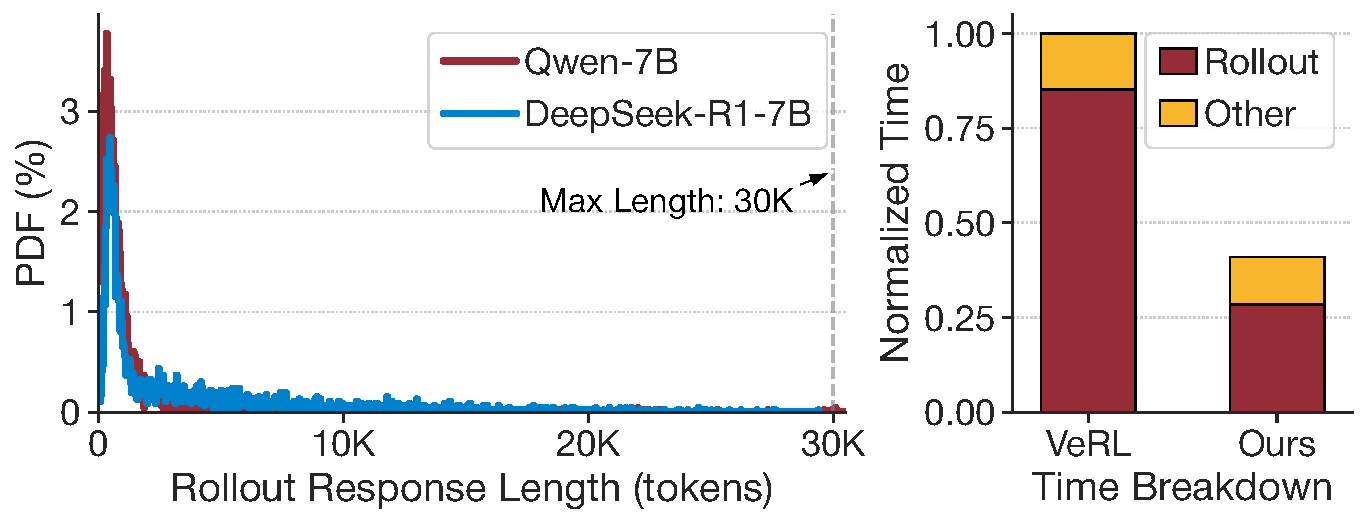
\includegraphics[width=\linewidth]{figures/motivation_distribution.pdf}
    \caption{响应长度分布与 RL 步骤时间分解。}
  \end{subfigure}
  \begin{subfigure}[b]{\linewidth}
    
\includegraphics[width=\linewidth]{figures/teaser.pdf}
    \caption{使用与不使用 \SysName 时推理 RL 步骤时间线的示意图。}
  \end{subfigure}
  \caption{推理 RL 中观测到的长尾生成（rollout）与工作负载不均衡问题。\SysName 通过自适应草稿模型有效应对这些挑战。}
  \label{fig:teaser}
\end{figure}

\section{引言}
\label{sec:intro}

过去一年间，我们见证了 OpenAI-o1~\cite{O1}、DeepSeek-R1~\cite{DeepSeekR1} 和 Gemini-2.5Pro~\cite{Gemini2.5Pro} 等推理 LLM 的出现；它们在数学推理、编程和多学科知识任务上展现出显著的能力提升~\cite{ReasoningSurvey}。这些进展的一个关键驱动力是强化学习（RL）：它已经成为赋予 LLM 强大推理能力的标准方法~\cite{DeepSeekMath,QwQ,DeepSeekR1,DAPO}。然而，相关工作负载具有独特特征，使这种 RL 方法面临效率挑战。我们分析自行采集的轨迹（图~\ref{fig:teaser}）以及 ByteDance 的生产轨迹（图~\ref{fig:bytedance}），识别出推理 RL 过程的以下关键特征。

\noindent\textbf{（1）Rollout 与训练时间不均衡。}
在 RL 中，第一个阶段也是最耗时的阶段是\emph{rollout}，模型在此生成大量候选响应。随后，这些响应被用于\emph{推理}和\emph{训练}阶段，以更新模型。如图~\ref{fig:teaser}(a) 所示，rollout 阶段占总步骤时间的比例异常之高（约 $85\%$），因而成为主要瓶颈。

\noindent\textbf{（2）持续存在的长尾分布。}
RL 训练低效的一个主要来源，是 rollout 响应长度的\emph{长尾分布}。如图~\ref{fig:teaser}(a) 所示，尽管绝大多数生成序列相对较短，仍有少量序列延伸到极端长度。关键在于，这种低效并非偶发现象；ByteDance 的生产轨迹（图~\ref{fig:bytedance}）表明，它会贯穿长期训练而持续出现。在大多数 RL 步骤中，少数响应达到配置的最大长度，而大多数响应明显更短。最大长度与第 75 百分位数（p75）之间的巨大差距，凸显了严重的资源利用不足。Berkeley~\cite{deepscalerTrace}、Alibaba~\cite{gao2025rollpacker} 和 AMD~\cite{zhou2025april} 的大规模 RL 系统也分别报告了相似的长尾模式，说明这一现象广泛存在。

\noindent\textbf{（3）巨大的时间与资源需求。}
图~\ref{fig:bytedance} 显示，即便使用 128 张 GPU，一个 32B 模型的推理 RL 训练仍耗时 11 天，却只完成 385 步。单个训练步骤平均约需 40 分钟，而每 5 步进行一次的周期性评测每次约需 20 分钟，说明该过程极其耗时、耗费资源。

现有 RLHF（基于人类反馈的强化学习）系统~\cite{HybridFlow,RLHFuse,ReaLHF,DeepSpeedChat,GEAR,NeMoAligner,FlexRLHF}主要优化多模型管理、数据传输以及跨阶段设备分配，却忽视了 rollout 瓶颈，因此对推理 RL 任务仍不够高效。更关键的是，推理 rollout 往往比典型 RLHF 输出长一个数量级以上~\cite{HybridFlow,RLHFuse,InstructGPT}，这使推理 RL 具有根本不同的工作负载特征，也要求不同的系统级优化。

尽管 LLM 服务已有多种加速技术，其中许多并不适合 RL 训练场景。例如，量化~\cite{AWQ,GPTQ}和模型稀疏化~\cite{LLM-Pruner,StreamingLLM}虽能带来加速，却通常是\emph{有损的}，可能降低模型准确率并改变输出概率。我们认为推测解码（Speculative Decoding，SD）~\cite{SpeculativeDecoding,chen2023accelerating}非常适合这一场景。SD 先用轻量草稿模型推测性地产生 token 序列，再由主目标模型并行验证。它尤其适合 RL 训练，原因有二：（1）\emph{数学上无损}：输出分布与原始目标模型的分布完全一致；（2）\emph{适合长尾}：SD 将过程从受显存带宽限制转向更受计算限制，从而提升吞吐；这对 RL rollout 的长尾阶段尤其有效，因为此时有效批大小通常较小。

然而，现有推测解码技术~\cite{Medusa,Eagle1,SpecInfer,HASS,Falcon,REST}面向目标模型固定的静态推理场景。把它们用于动态的推理 RL 训练并非简单移植，而会遇到三项重大挑战：（1）\emph{目标模型持续演化}：RL 训练不断更新目标模型权重，使草稿模型日益“陈旧”，严重削弱 SD 效果；（2）\emph{草稿模型训练成本}：高效 SD 通常依赖专门的草稿模型~\cite{HASS,Eagle1,Eagle2,Eagle3,Falcon,Hydra}，为目标模型训练并对齐草稿模型会给用户增加开销与复杂度；（3）\emph{调度复杂}：SD 性能对批大小以及草稿深度等超参数十分敏感，但推理 RL rollout 的有效批大小会随序列在不同时刻完成而动态波动，因此需要有效的策略选择器。

为解决这些挑战，我们提出 \SysName，一个具备自适应推测解码能力的高效推理 RL 训练系统。\SysName 旨在缓解长尾 rollout 瓶颈，同时保证数学上的无损性。其核心设计来自两点洞察。第一，\emph{利用 rollout 气泡}：RL rollout 特有的长持续时间，为使用因长尾效应逐步释放的 GPU 资源提供了充足窗口。随着序列完成而释放的资源可以改用于草稿模型训练等其他任务，且不产生额外成本~\cite{Hydro}。第二，\emph{非阻塞式草稿器训练}：草稿模型训练可以与完整 rollout 的完成解耦；在部分数据或随时可用的数据上异步训练，可以把其计算与仍在进行的 rollout 有效重叠。

\begin{figure}[t]
  \centering
  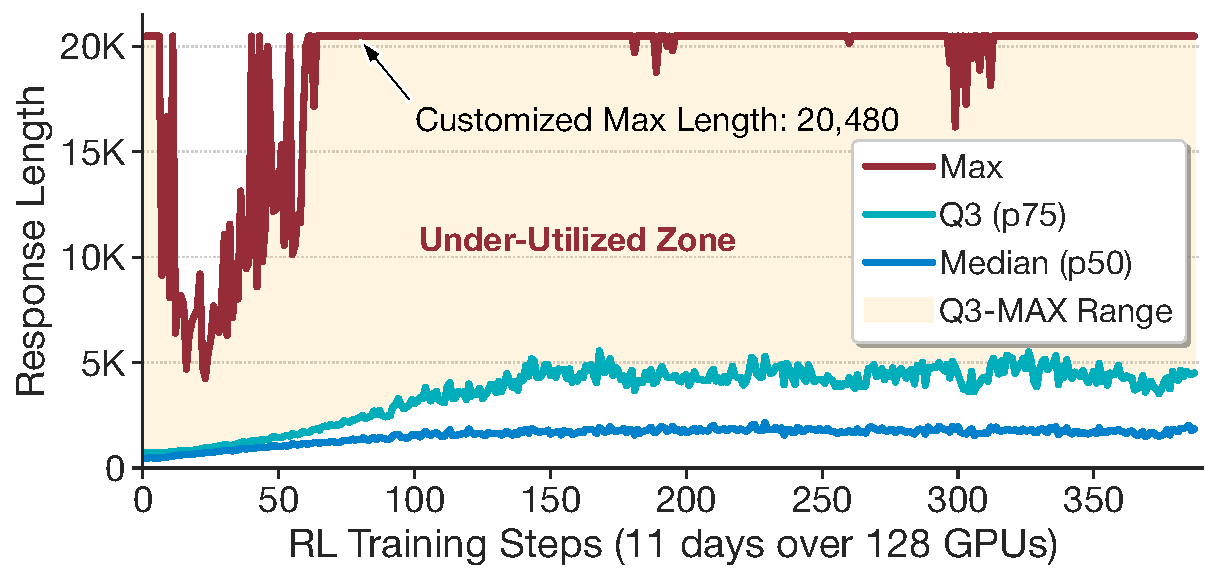
\includegraphics[width=\linewidth]{figures/bg_and_motiv/response_length_distribution.pdf}
  \caption{ByteDance 的 RL 训练轨迹~\cite{dapoTrace}，基于 Qwen2.5-32B~\cite{qwen25}并在 H20 96GB GPU 上执行。“p75”表示第 75 百分位数；原始来源未提供更细粒度的百分位数据。}
  \label{fig:bytedance}
\end{figure}

基于以上洞察，我们以多项系统优化构建 \SysName：（1）自适应草稿模型（第~\ref{sec:drafter} 节）：我们采用轻量草稿模型，并通过 spot trainer 持续适配，创新性地处理 RL 训练中目标模型不断演化的问题。该训练器利用长尾 rollout 期间的空闲 GPU 资源，以机会式、可抢占的方式更新草稿器，从而在不增加开销的情况下保持其与目标模型一致。（2）自适应 Rollout 引擎（第~\ref{sec:engine} 节）：\SysName 维护显存高效的预捕获 CUDAGraph 池，并使用 BEG-MAB 调优器为每个输入批自适应选择适合的 SD 策略；在早期 rollout 步骤中，它还支持无模型推测解码。

图~\ref{fig:teaser}(b) 直观展示了 \SysName 的工作流：系统自动利用空闲资源（例如 worker W3--W5）进行机会式草稿模型训练（蓝色方块），从而抵消目标模型更新造成的性能下降，且不增加额外成本。同时，\SysName 在这些资源利用不足的时段自适应启用推测解码（蓝色斜线方块），以进一步提高效率。

通过协同结合自适应草稿模型与协调式调度，\SysName 有效缓解了 RL 训练固有的长尾问题。我们在多种模型架构和真实数据集上评测 \SysName。实验表明，它在保持模型输出质量、尽量减少资源浪费的同时，显著提高了端到端训练吞吐。此外，该过程还免费产出可供后续部署使用的有效草稿模型。

\section{背景与动机}
\label{sec:background}

\subsection{推理与强化学习}

\begin{figure}[t]
  \centering
  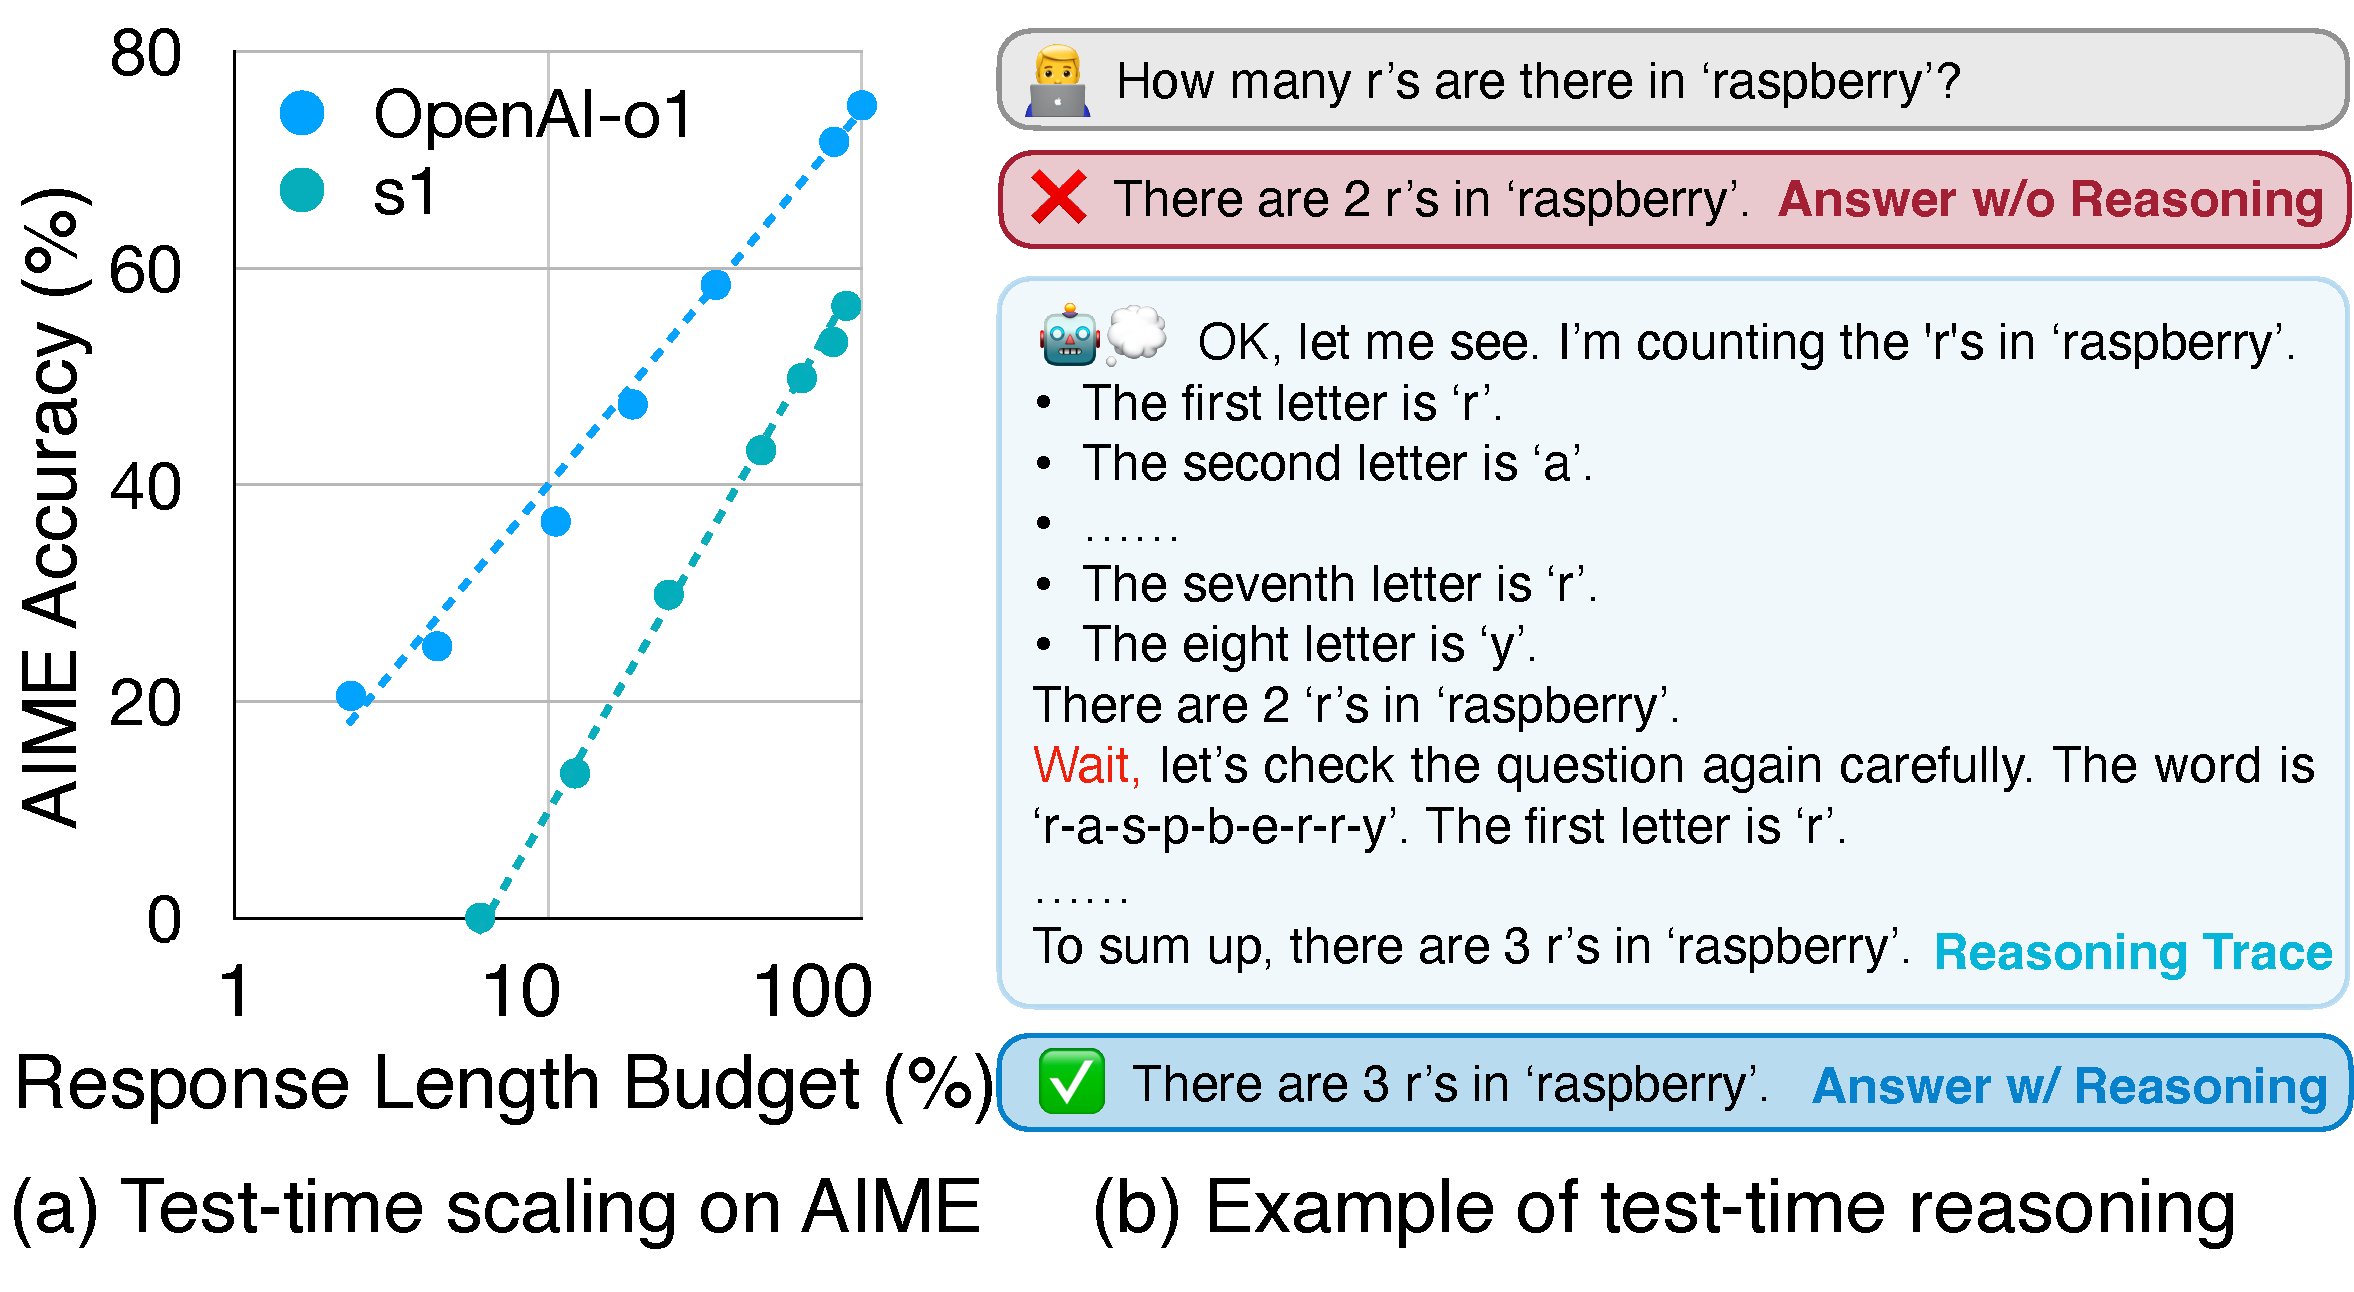
\includegraphics[width=\linewidth]{figures/bg_and_motiv/test_time_scale.pdf}
  \caption{推理模型的\textbf{测试时扩展}。（a）OpenAI-o1~\cite{O1}与 Stanford s1-32B~\cite{s1}在 AIME 竞赛级数学基准~\cite{AIME}上的表现。（b）推理过程中通过自我反思纠正错误的示例。}
  \label{fig:test-time}
\end{figure}

\noindent\textbf{推理 LLM。}
大语言模型近期在数学、逻辑与编程等复杂推理领域展现出卓越表现。OpenAI-o1~\cite{O1}和 DeepSeek-R1~\cite{DeepSeekR1}等强大模型在竞赛级数学与编程挑战等困难推理基准上取得了令人印象深刻的准确率。它们成功的关键因素之一是\emph{测试时扩展}~\cite{InferenceScalingLaws,GreedyPolicySearch}：这种推理范式为模型提供更多生成时间以探索复杂推理路径，从而提高准确率。

这些推理 LLM 通常具有两项特征：（1）\emph{长思维链}：在得到最终答案之前，生成较长的中间推理步骤；（2）\emph{自我反思}：能够在推理期间评估、改进并纠正自己的推理，从而提升准确率。如图~\ref{fig:test-time}(a) 所示，延长生成时间使这些模型能够探索更深、更广的思维轨迹~\cite{ReasoningSurvey}，无需额外训练成本即可提高准确率。更重要的是，与传统 LLM 不同，这些推理模型会自动回顾已生成的响应，并表现出自我反思能力，例如图~\ref{fig:test-time}(b) 推理轨迹中的“wait”。这种能力通常在 RL 训练阶段获得~\cite{DeepSeekR1}，也是性能提升的关键。

\begin{figure}[t]
  \centering
  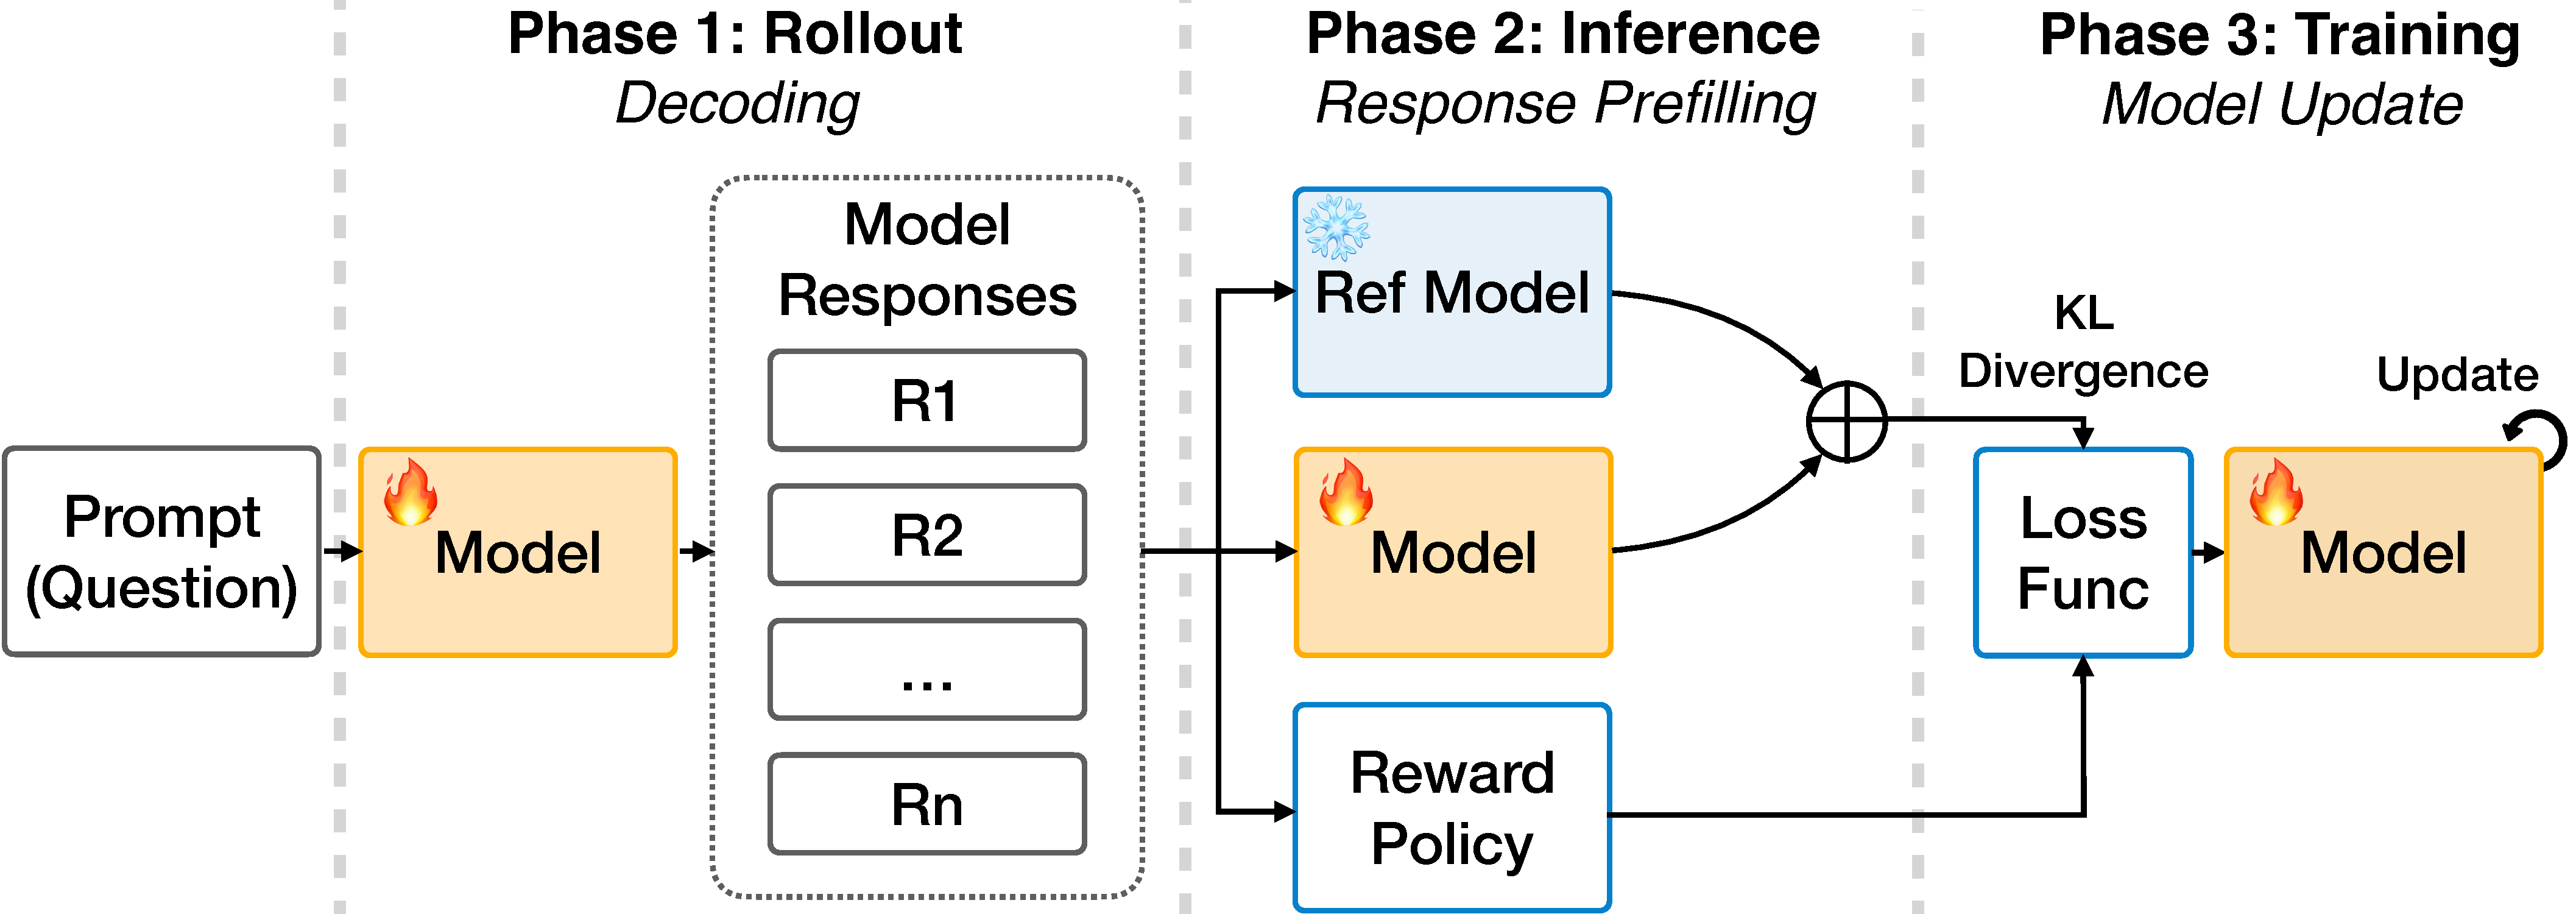
\includegraphics[width=\linewidth]{figures/bg_and_motiv/rl_overview.pdf}
  \caption{GRPO~\cite{DeepSeekMath}强化学习训练流程概览。}
  \label{fig:grpo}
\end{figure}

\noindent\textbf{用于推理的强化学习。}
近期，组相对策略优化（GRPO）~\cite{DeepSeekMath}等 RL 算法变体已被证明能成功训练推理 LLM。与依赖大型 critic 模型的标准近端策略优化（PPO）~\cite{PPO}不同，GRPO 使用基于组的基线估计来简化优化过程，在保持策略更新稳健性的同时显著降低训练开销~\cite{PostTrainingSurvey}。

图~\ref{fig:grpo} 展示了 GRPO 的一个训练步骤，其中包含三个主要阶段：（1）\textbf{rollout 阶段}：目标模型为每个输入提示生成多个候选响应；（2）\textbf{推理阶段}：生成的响应同时由\textsl{目标模型}（正在接受 RL 训练的模型）和固定的\textsl{参考模型}（初始目标模型，即 RL 步骤为 0 时的模型）处理。处理得到的 logits 用于计算 KL 散度惩罚~\cite{john2020kld}，它约束模型更新，保证训练稳定并防止模型过度偏离参考模型。与此同时，该阶段还根据响应特征（例如正确性）按\emph{基于规则}的策略计算奖励，而不依赖单独的价值模型；（3）\textbf{训练阶段}：使用奖励值和 KL 散度构造损失函数，再根据该损失更新目标模型权重。

\subsection{以推测解码实现高效推理 RL}
\label{sec:sd-background}

\begin{figure}[t]
  \centering
  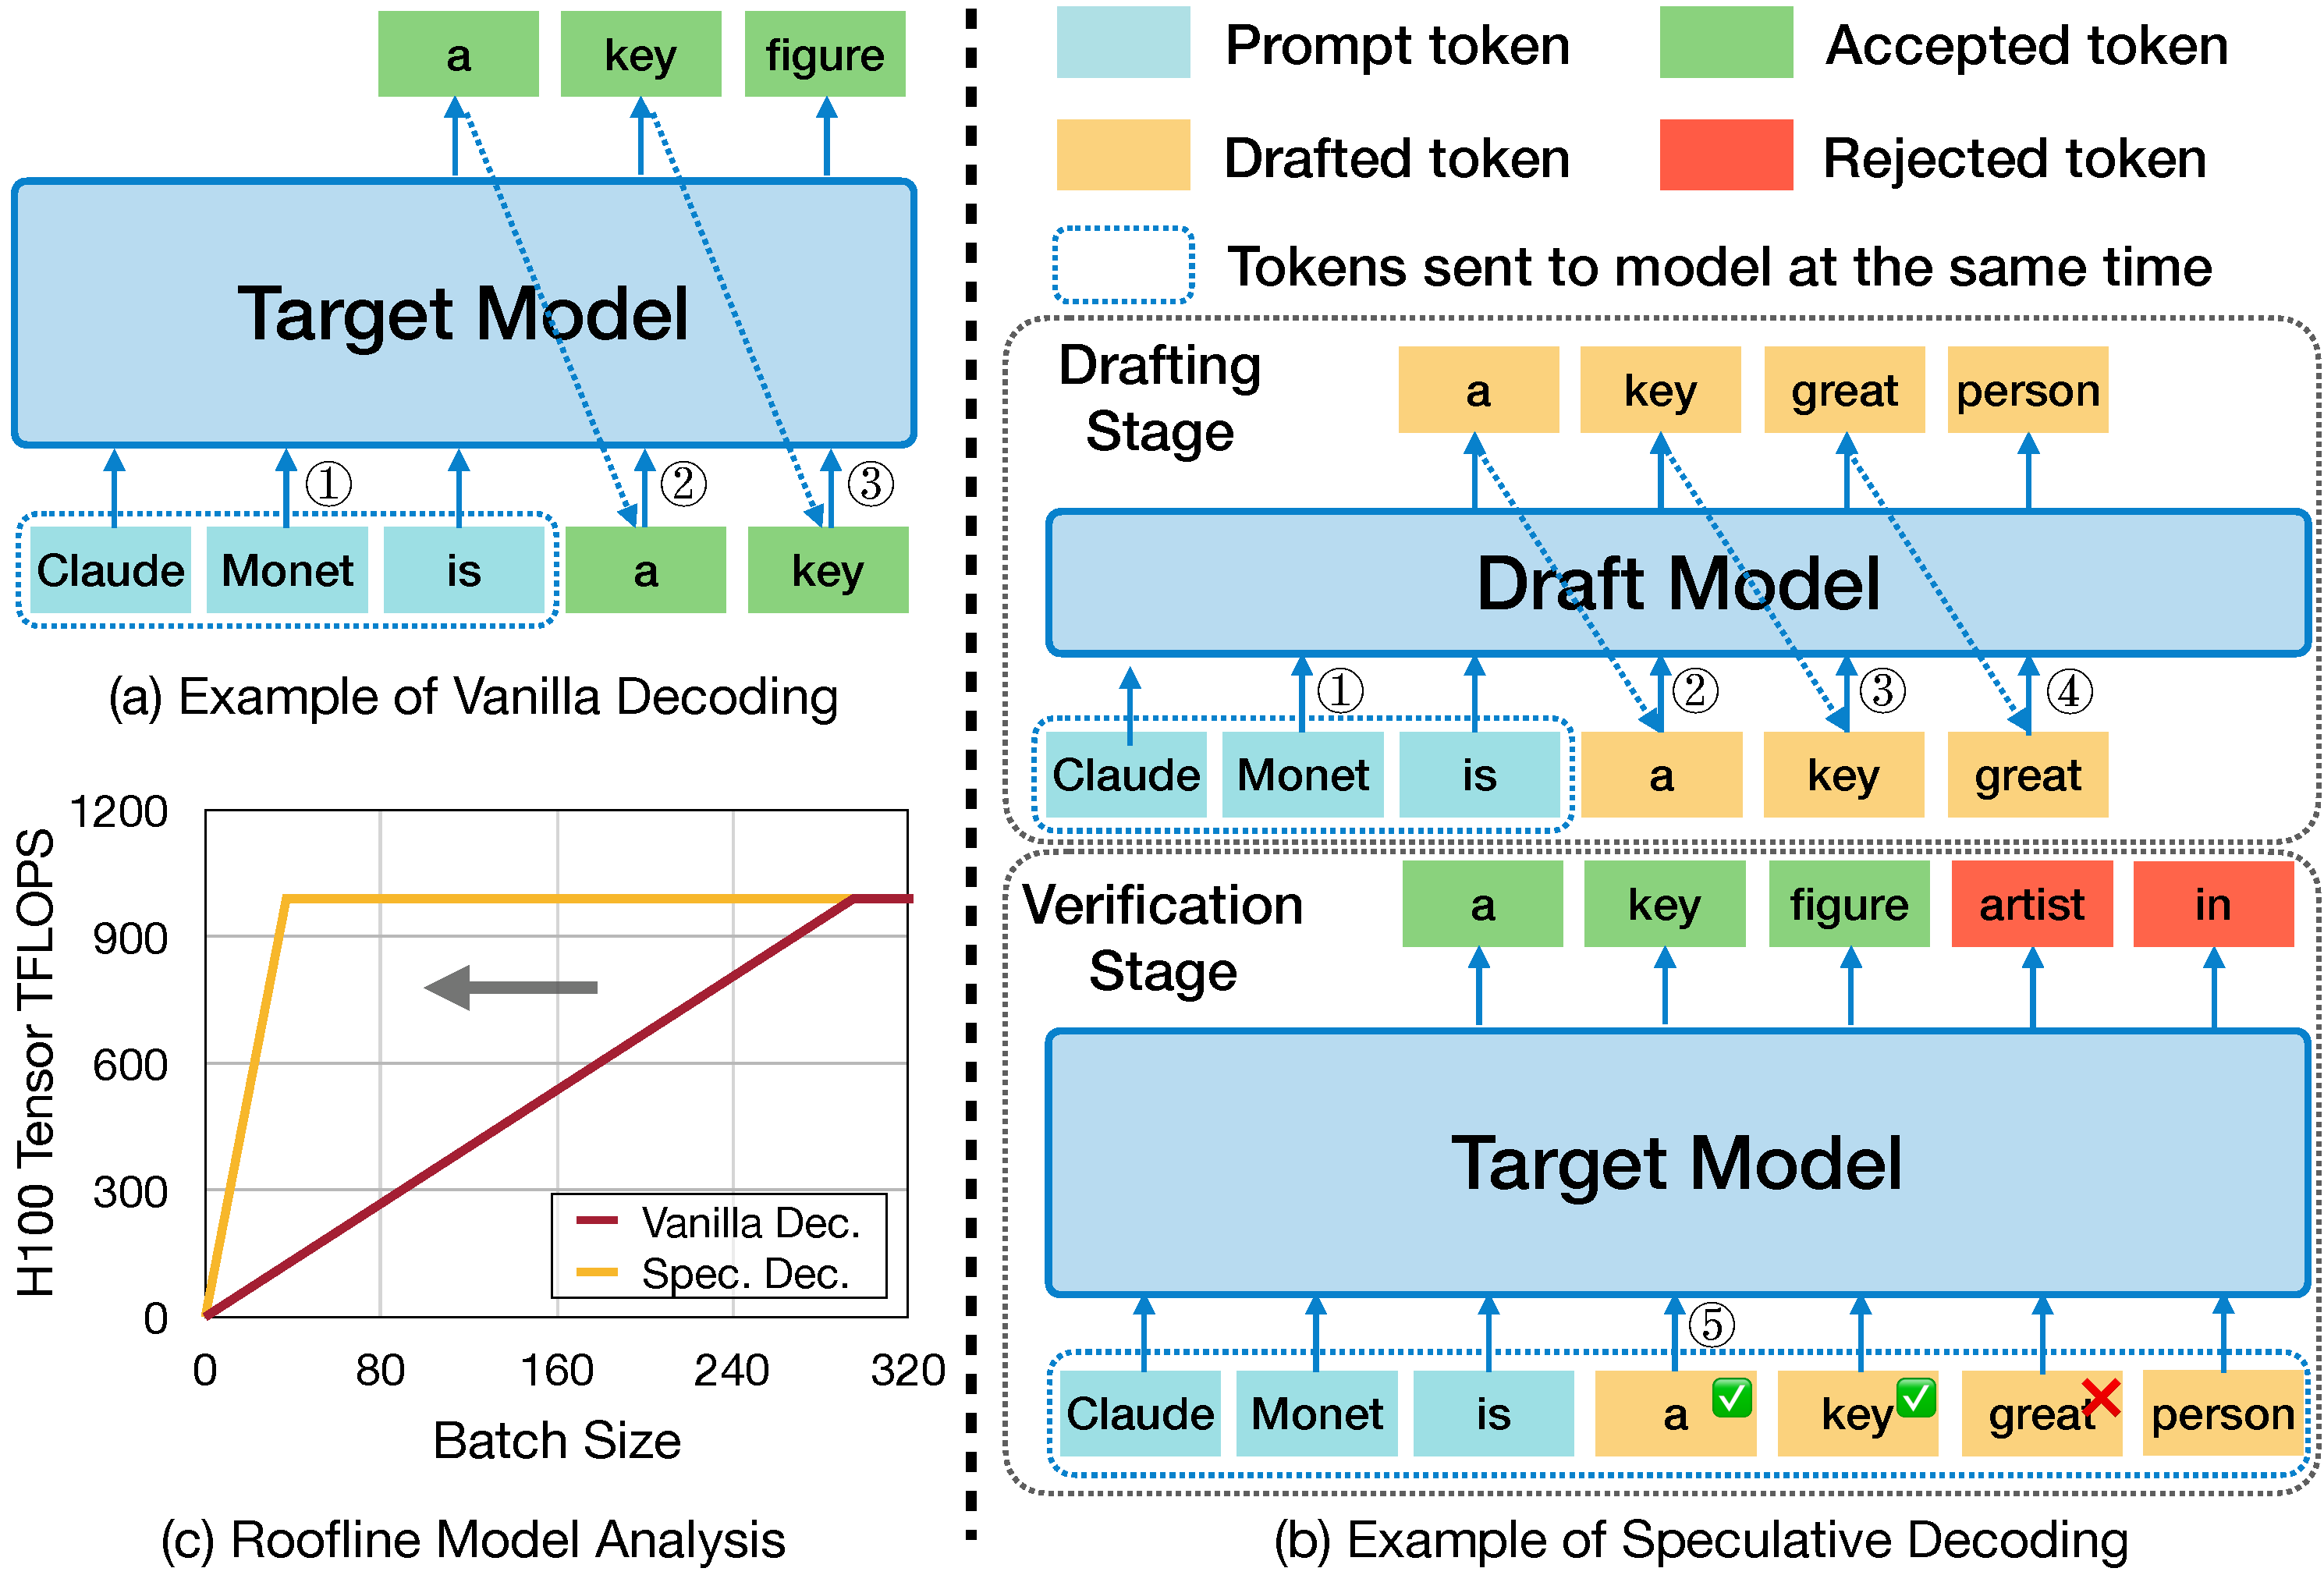
\includegraphics[width=\linewidth]{figures/bg_and_motiv/spec_dec.pdf}
  \caption{\textbf{推测解码概览。}（a、b）普通解码与推测解码的比较。（c）推测解码在显著更小的批大小下即可达到峰值计算吞吐（TFLOPS，灰色箭头）。}
  \label{fig:sd}
\end{figure}

如第~\ref{sec:intro} 节所述，推理 RL 的长尾 rollout 阶段经常成为性能瓶颈。因此，要提高吞吐和资源效率，就必须针对解码加速设计专门的系统优化。为此，我们将推测解码~\cite{SpeculativeDecoding,chen2023accelerating}确定为很适合解决这些挑战的关键方法。

\begin{figure*}[t]
  \centering
  
\includegraphics[width=.95\textwidth]{figures/main.pdf}
  \caption{\SysName 的整体架构与工作流。}
  \label{fig:system}
\end{figure*}

\noindent\textbf{为何采用推测解码。}
在众多 LLM 解码加速方法中，推测解码尤其适合推理 RL 场景。它最主要的优势是\emph{无损}：在数学上保证输出分布与原目标模型完全相同。对于推理任务，这种保真性至关重要，因为生成步骤的正确性与逻辑连贯性是有效强化学习的基础。SD 通过加快生成直接处理长尾 rollout 阶段的吞吐瓶颈；它提高样本生成效率，同时不牺牲可靠推理 RL 训练所必需的准确率。

\noindent\textbf{推测解码的机制。}
在推测解码中（图~\ref{fig:sd}(b)），轻量草稿模型快速生成一串候选 token，随后更大的目标模型在一次前向传播中并行、高效地验证这些候选。系统接受草稿序列中首次与目标模型预测不匹配之前的全部 token，同时保留目标模型在该位置生成的一个正确 token。如图~\ref{fig:sd}(c) 的屋顶线分析所示，这一过程把通常受显存带宽限制的自回归生成转向更受计算限制的操作，更充分地占用 GPU 资源，从而提升吞吐。

\noindent\textbf{推理 RL 中的挑战。}
尽管 SD 能有效缓解显存带宽瓶颈并提高解码吞吐，但把现有方法适配到 RL 训练仍绝非易事。我们识别出三项关键挑战。

\textbf{C1：不断演化的目标模型。}不同于模型固定的标准推理场景，RL 训练会持续更新目标模型。这种不断演化使 SD 使用的草稿模型逐渐“陈旧”，降低推测 token 的接受率，并显著削弱 SD 的有效性。

\textbf{C2：草稿模型的训练成本。}要取得高 SD 效率，往往需要专用草稿模型，例如 Eagle~\cite{Eagle1}和 HASS~\cite{HASS}中的单解码层模型，而不能任意选择一个较小模型。为目标模型训练专用草稿器会带来可观的额外成本。

\textbf{C3：波动的批大小。}如图~\ref{fig:sd}(c) 所示，SD 通常针对小批量优化；RL rollout 的生成批大小却经常动态变化。若缺乏妥善管理，大批量下的性能可能下降，因此难以在这种场景中高效应用 SD，并会影响整体吞吐。

为解决这些挑战，\SysName 利用推理 RL 训练流程的独特特征。具体而言，我们引入自适应草稿模型（第~\ref{sec:drafter} 节）以缓解动态模型权重造成的性能下降（\textbf{C1}），利用空闲 GPU 资源高效更新草稿模型，从而消除训练开销（\textbf{C2}）。此外，我们在推理 RL 系统内设计专门的调度策略（第~\ref{sec:engine} 节），有效管理批大小变化带来的挑战（\textbf{C3}）。

\section{\SysName 概览}
\label{sec:overview}

\noindent\textbf{设计原则与目标。}
为了便于实际采用，\SysName 遵循四项关键设计原则：（a）\emph{无损保证}：与原始算法相比，系统优化必须在 rollout 与训练阶段都保持数学等价，避免异步陈旧性或有损近似；（b）\emph{无干扰}：自适应草稿器的工作负载不得干扰主要 RL 工作负载。草稿器更新以机会式 spot 任务执行，并可平滑抢占，以尽量减小对 RL 工作负载的影响；（c）\emph{自动且简单}：手动设置草稿模型及其推测超参数既繁琐，又常导致次优性能，因此 \SysName 提供自动化工作流以简化使用；（d）\emph{可泛化且可扩展}：设计必须适配 GRPO~\cite{DeepSeekMath}、RLOO~\cite{RLOO}等常用推理 RL 算法，并能随模型规模、架构和集群规模变化而有效扩展，持续带来系统性能提升。

此外，\SysName 有三个主要目标：（1）缓解长尾问题，加速推理 RL 训练；（2）提高集群利用率，尽量减少资源浪费；（3）无需额外成本即可产出高性能草稿模型，用于未来的推测解码部署。

\noindent\textbf{架构与工作流。}
图~\ref{fig:system} 展示了 \SysName 的整体架构和工作流。系统由两个紧密集成的组件组成：自适应草稿模型（第~\ref{sec:drafter} 节）和自适应 Rollout 引擎（第~\ref{sec:engine} 节）。

rollout 过程有两个关键特征：序列长度呈长尾分布，并且随着响应完成，批大小逐渐缩小。为适应这些动态变化，自适应 Rollout 引擎为目标模型和草稿模型维护预捕获 CUDAGraph 池，并由自适应 SD 管理器进行管理。该管理器使用本文提出的 BEG-MAB 调优器，自动为每个输入批选择合适的 SD 策略。如图~\ref{fig:system} 顶部所示，被选中的草稿器 CUDAGraph 生成候选 token，随后传给相应的目标 CUDAGraph 并行验证。引擎测量接受长度与步骤延迟，再把这些信号反馈给 SD 管理器，以实时改进策略选择。

与此同时，自适应草稿器模块负责持续更新轻量草稿模型，且不干扰主要 rollout 工作负载。集中式 Worker Coordinator 监测 rollout worker 的状态。当长尾阶段出现空闲资源时，协调器便机会式地启动 Spot Trainer 任务。训练任务使用 Online DataBuffer，其中缓存当前和先前步骤 rollout 的隐藏状态与输入 embedding。系统通过无填充打包和选择性异步检查点等技术高效更新草稿模型。这一设计确保草稿器更新可被无缝抢占与恢复，从而利用原本浪费的资源气泡。

通过系统性地结合自适应 rollout 和机会式草稿器训练，\SysName 在不牺牲模型质量的情况下显著加速推理 RL，并免费产出有价值的草稿模型。

\section{自适应草稿模型}
\label{sec:drafter}

\begin{figure}[t]
  \centering
  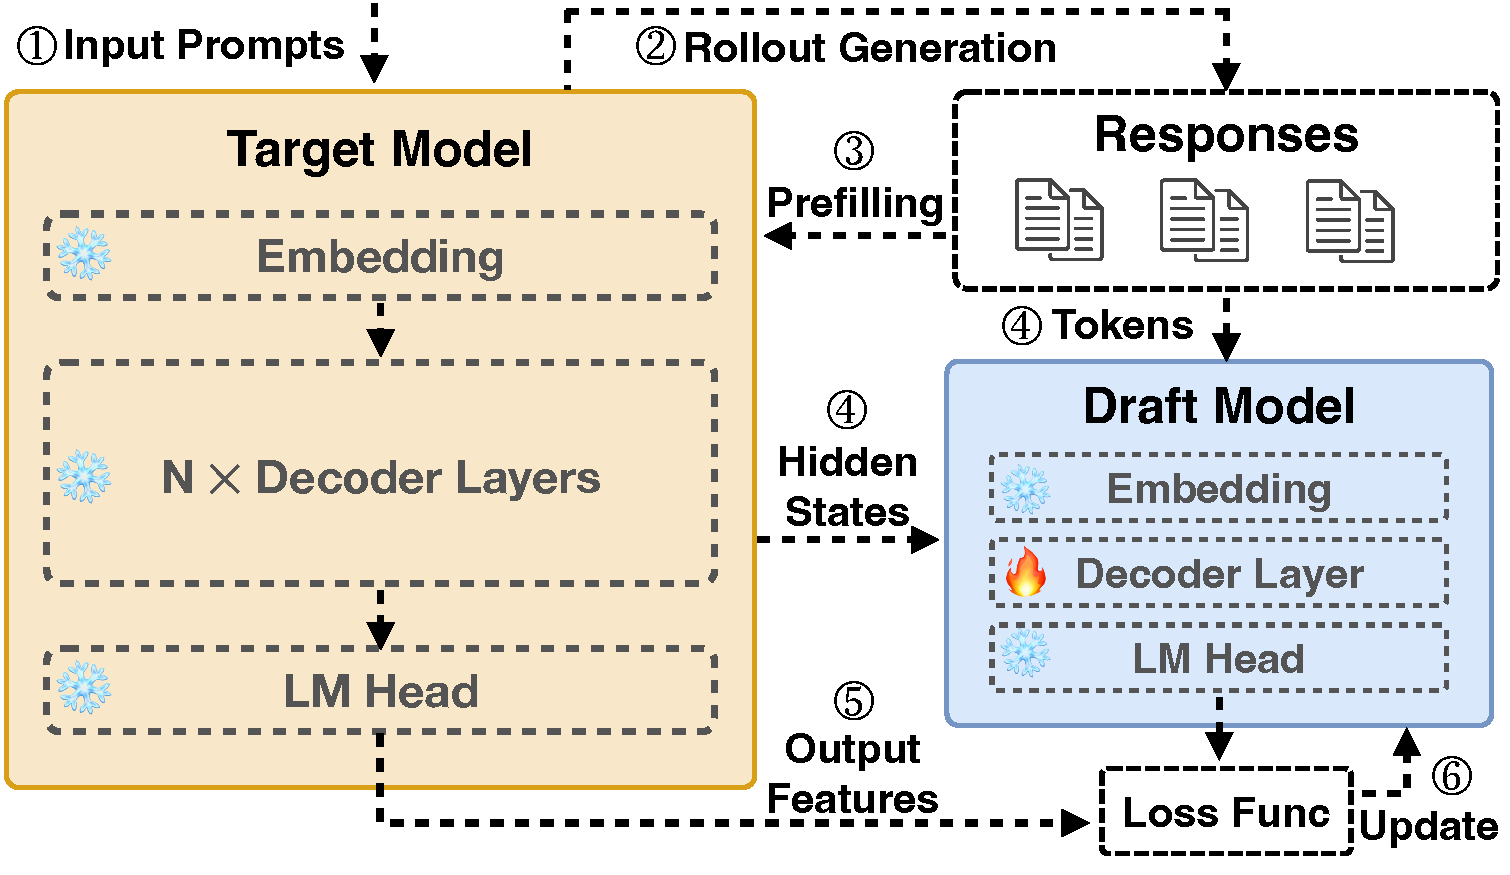
\includegraphics[width=\linewidth]{figures/method/draft_trainer.pdf}
  \resizebox{\linewidth}{!}{%
  \begin{tabular}{@{}lccc@{}}
    \toprule
    策略 & 隐藏状态 & 损失函数 & 训练时测试 \\
    \midrule
    Eagle~\cite{Eagle1} & 最后一层 & L1 + CE & 不适用 \\
    HASS~\cite{HASS} & 最后一层 & L1 + CE & 3 步 \\
    Eagle-3~\cite{Eagle3} & 顶层、中层和底层 & 仅 CE & 7 步 \\
    \bottomrule
  \end{tabular}}
  \caption{\textbf{草稿模型训练。}上：使用目标模型隐藏状态的统一训练流程。下：不同训练策略的具体配置。}
  \label{fig:draft-training}
\end{figure}

本节介绍 \SysName 的自适应草稿模型组件，重点说明它如何创建、训练和使用草稿模型，在不干扰主要 RL 工作负载的前提下加速推理 RL 过程。

\subsection{草稿模型}

\SysName 使用经过专门训练的紧凑模型来模仿目标 LLM 的 token 生成行为，从而实现高效、准确的推测执行。

\noindent\textbf{模型架构。}
为最大化效率，\SysName 为草稿器采用高度轻量的\emph{单层}模型设计~\cite{Eagle1,HASS,Eagle3}。这里的“一层”指包含注意力和前馈组件的完整 Transformer decoder block。这与普通推测解码~\cite{SpeculativeDecoding,chen2023accelerating}不同，后者往往从同一模型家族另取一个更小的多层 LLM，例如为 Qwen2.5-32B 目标模型使用 Qwen2.5-0.5B。普通方案存在缺点：并非每个目标 LLM 都有合适且准确的小型草稿器，而且这些较小模型仍可能产生可观的草拟延迟。以 Qwen2.5 为例，32B 模型有 64 层，而 0.5B 模型仍有 24 层。尽管参数量在此例中减少了 $64\times$，延迟仍由多层间的顺序计算主导。实验表明，\SysName 的单层草稿模型与 Qwen2.5-0.5B 草稿器参数量大致相同，却快 $2.4\times$。

如图~\ref{fig:draft-training} 蓝色方块所示，\SysName 草稿器沿用目标模型架构，但只包含一个可训练的 decoder 层。它复用目标模型原有的 Embedding 和 LM Head 层，并在训练期间冻结其权重。因此，系统只更新单个 decoder 层的参数，这些参数约占目标模型总参数的 $\texttt{1/layer\_num}$。这一架构显著降低训练和推理开销。已有研究~\cite{HASS,Eagle1,Eagle2,Eagle3,Falcon,Hydra}也验证了这种单层草稿器的有效性：它们能紧密对齐目标模型的自回归分布，并对推测 token 取得较高接受率。运行时，训练后的草稿器接收目标模型的隐藏状态，并以自回归方式草拟后续 token，供目标模型验证。

\noindent\textbf{训练过程。}
\SysName 构建了支持多种草稿模型训练策略、并与 RL 工作流无缝集成的统一训练框架。如图~\ref{fig:draft-training} 所示，训练过程利用 RL 工作流产生的数据。具体来说，输入提示先由目标模型处理并生成 rollout 响应。随后的预填充（即推理）阶段从目标模型特定层收集隐藏状态。系统将这些隐藏状态与输入 token embedding 拼接，再通过轻量线性层降维，所得输出特征便作为输入来训练草稿器的单个 decoder 层。目标模型比草稿模型大得多（超过 $20\times$），其预填充成本可能远高于一次草稿器训练迭代。\SysName 把 RL 固有推理阶段产生的隐藏状态缓存到主机内存并加以复用，从而消除这部分开销。

\SysName 还支持多种训练目标：框架可以对目标模型和草稿模型的隐藏状态施加 L1 损失以对齐表示，可以对输出 logits 施加交叉熵（CE）损失以匹配 token 预测，也可以组合两者。随后，计算得到的损失通过反向传播只更新草稿器的 decoder 层，Embedding 和 LM Head 仍与目标模型绑定。

由于该框架与具体草稿器无关，统一管线还支持多种训练策略。例如，EAGLE~\cite{Eagle1}只使用最后一层隐藏状态；HASS~\cite{HASS}把草稿模型的输出特征多次反馈给自身，即执行“训练时测试”，以进一步强化训练；EAGLE-3~\cite{Eagle3}则融合目标模型多个层级的隐藏状态，以争取更高接受率。尽管这些策略存在差异，都能自然表达在我们的训练框架中。本文默认使用 EAGLE，因为它能以低得多的训练成本取得较高接受长度和更快收敛。

\begin{figure}[t]
  \centering
  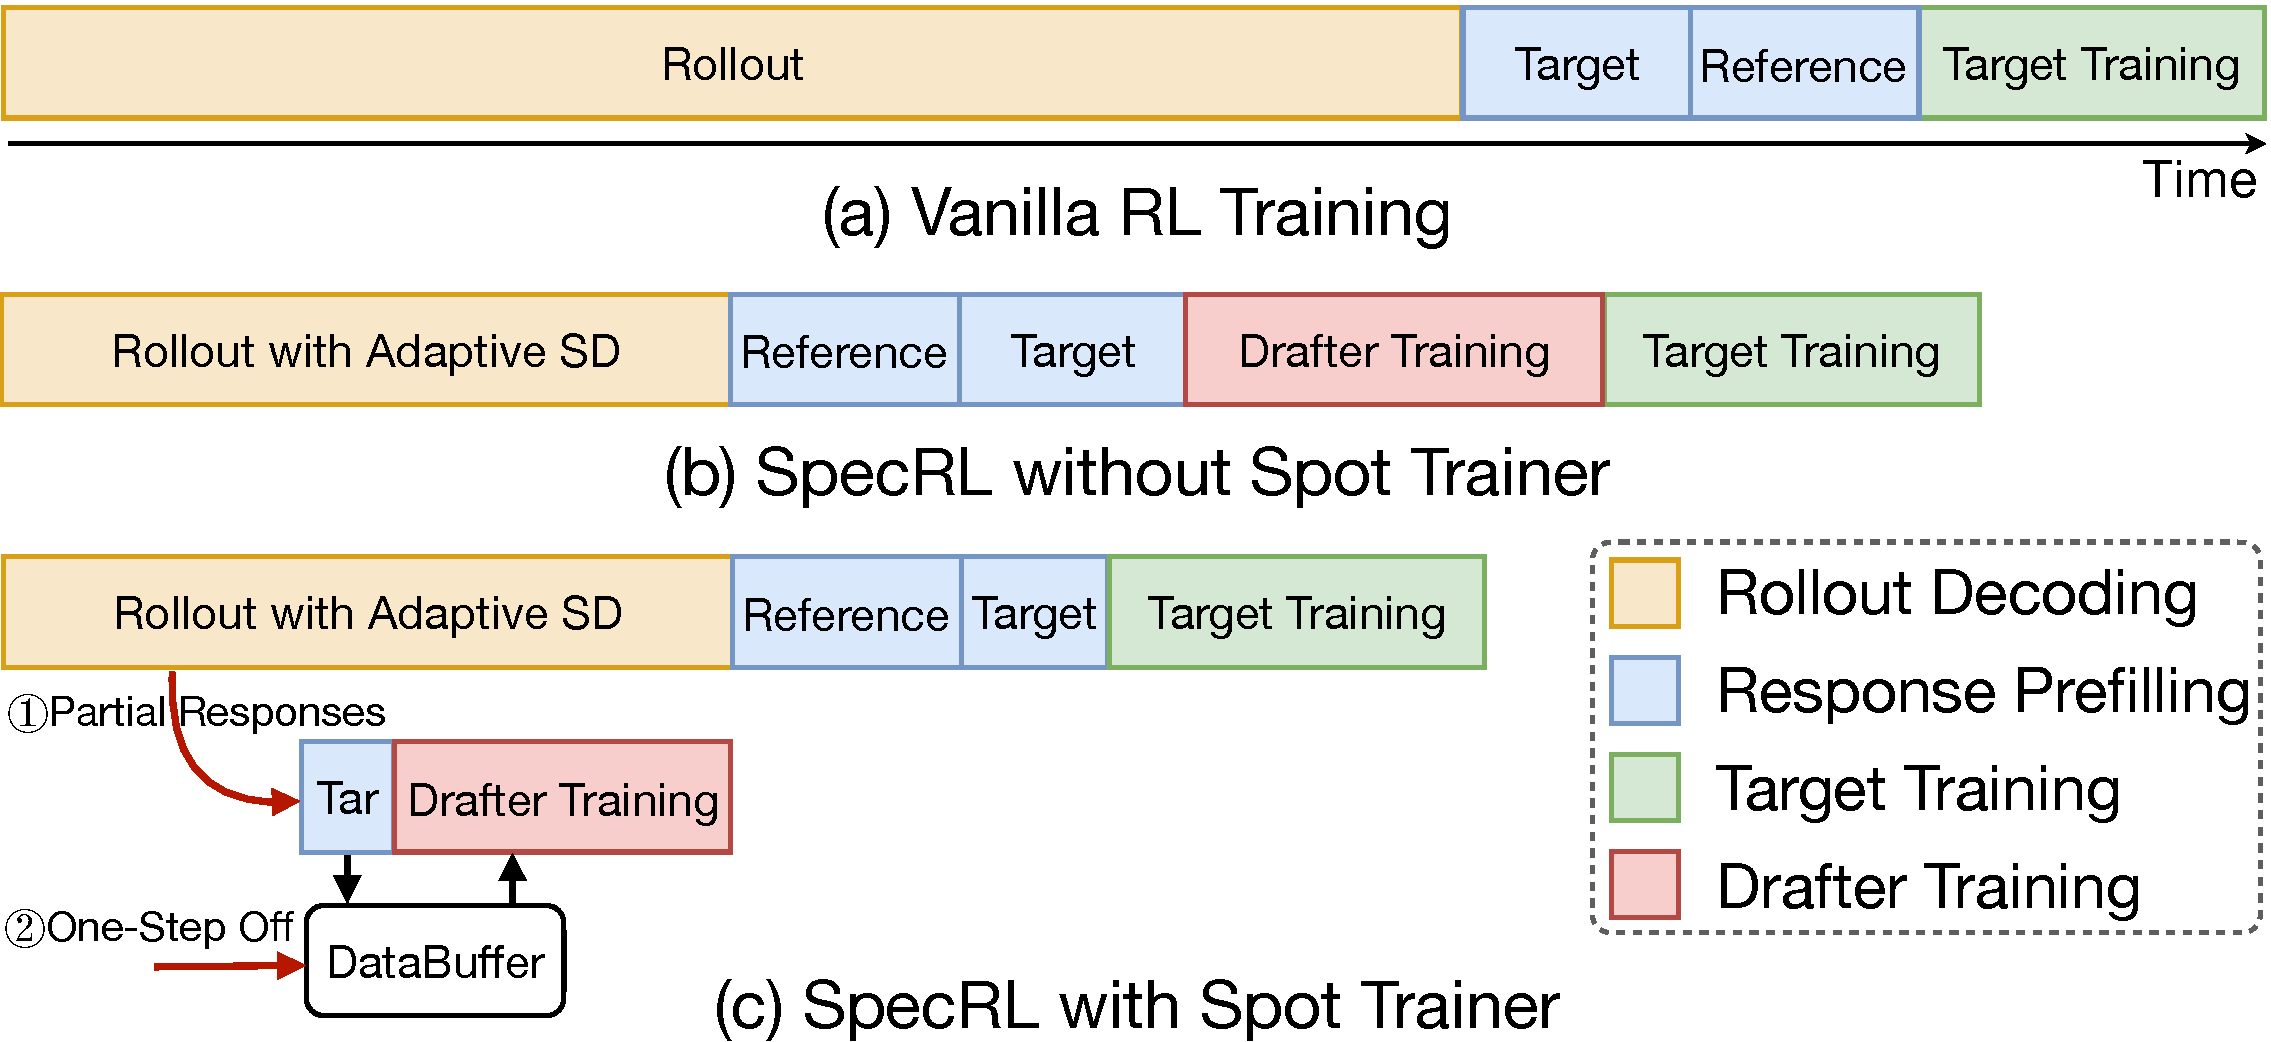
\includegraphics[width=\linewidth]{figures/method/waterfall.pdf}
  \caption{\textbf{Spot Trainer 工作流。}图中方块长度仅作示意，并不严格对应执行时间。草稿器训练中的目标模型预填充是可选的，因为可以直接使用 rollout 引擎提供的隐藏状态。}
  \label{fig:waterfall}
\end{figure}

\subsection{Spot Trainer}

在 RL 训练中应用推测解码的关键挑战是\emph{目标模型不断演化}（\textbf{C1}），这会使固定草稿模型迅速陈旧并失效。Spot Trainer 的设计目标是在不妨碍主要 RL 工作流的前提下抵消这种漂移。为此，\SysName 采用以下新设计。

\noindent\textbf{Worker Coordinator。}
协调器用于衔接 Rollout Engine 与 Spot Trainer，协调资源分配，尤其是重新利用 rollout 长尾阶段变为空闲的 GPU 资源。在 \SysName 中，\emph{worker} 是资源管理的基本单元，定义为一个 rollout 实例。例如，当 rollout 以 TP=8 使用完整 DGX-H100 节点时，一个 worker 就代表 8 张 GPU。协调器采用基于 ZeroMQ~\cite{ZeroMQ}实现的集中式模型：单个协调器进程（rank 0）维护全局状态，worker 通过异步请求--响应模式通信。协调器监测活跃请求数与 worker 状态，据此决定何时把 worker 从 rollout 迁移到机会式草稿器训练。每个 worker 在三种状态间循环：\emph{BUSY}（服务 rollout）、\emph{IDLE}（推理完成且显存已释放）和\emph{TRAINING}（进行草稿器更新），并在每次转换时通知协调器。当空闲 worker 数超过可配置阈值时，协调器将它们提升为训练模式并启动草稿器训练。

训练启动采用 leader election 模式：首个符合条件的 worker 建立训练会话；属于同一数据并行组的后续 worker 可以加入。rollout 完成时，协调器立即停止仍在进行的草稿器训练，并优雅关闭以确保正确清理。由此，系统能够有效利用长尾 rollout 期间的空闲 GPU 周期，而不干扰主要 RL 工作流。

\noindent\textbf{结合 DataBuffer 的 Spot Training。}
图~\ref{fig:waterfall} 对比了 Spot Trainer 与标准 RL 工作流。普通 RL（a）是顺序过程：rollout、目标模型和参考模型推理以计算 KL 散度、目标模型训练；奖励计算很快，图中为简洁起见省略。朴素集成草稿器训练（b）通常把它增加为另一个顺序步骤，尽管可以复用部分预填充计算，仍会产生额外开销。

与之不同，Spot Trainer（c）基于如下原则运行：草稿模型训练无需等待所有生成响应完成，也能有效推进，因此可用非阻塞方式执行。在推理 RL 任务的长尾分布下，大多数响应比最长响应早得多生成完毕。Spot Trainer 利用这一观察，以部分响应训练草稿模型。然而，若只依赖提前完成的响应，草稿器很少见到极长序列，可能造成分布失配。为此，\SysName 引入 \textbf{DataBuffer}，使草稿器训练与 rollout 完成解耦。DataBuffer 缓存推理阶段产生的隐藏状态和 token，并以极低开销加载它们。关键在于，它支持\emph{一步偏移}采样：缓冲区跨 RL 步持久保留，并优先采样前一步的长序列，以补偿当前部分数据中长尾样本的稀缺。尽管这些样本略有陈旧，对草稿器训练仍然有效。实验显示，把当前步骤的部分数据与缓冲的长序列结合起来，可以达到与完整响应集训练相当的性能。草稿器更新作为低优先级“spot 任务”调度到空闲 GPU 上，从而收获长尾释放的计算资源，同时保持主要 RL 工作流非阻塞。

\begin{figure}[t]
  \centering
  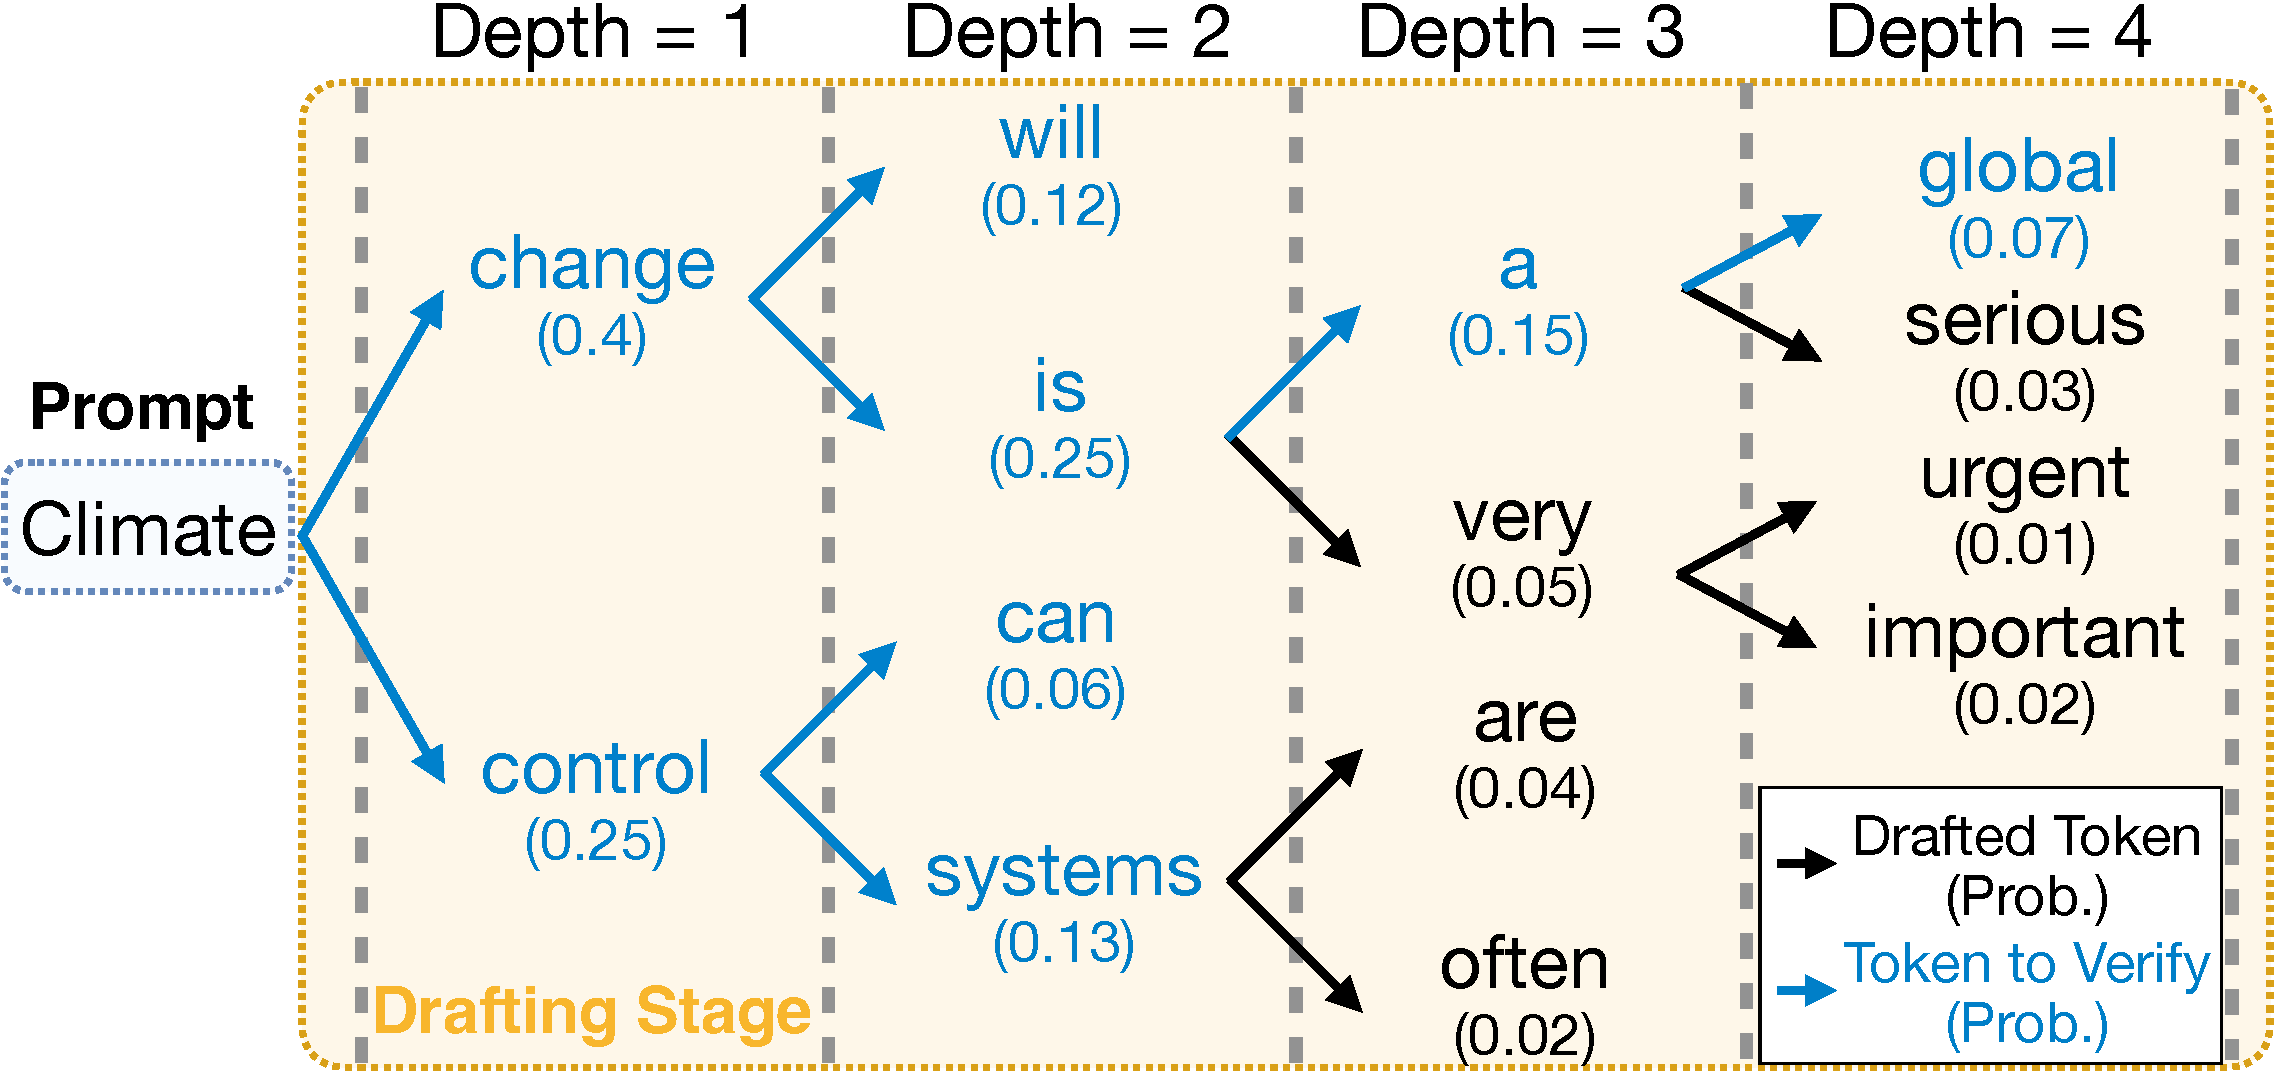
\includegraphics[width=.92\linewidth]{figures/method/tree_decoding.pdf}
  \caption{\textbf{树式解码示例。}本例设置 \texttt{topK=2}、\texttt{Draft\_Depth=4}、\texttt{Tokens\_to\_Verify=8}；Prob. 表示草稿模型给出的 token 概率。}
  \label{fig:tree}
\end{figure}

\noindent\textbf{选择性异步检查点。}
Spot Trainer 的一个关键设计特征是可抢占，使其能够使用空闲资源而不阻塞主要 RL 工作负载。然而，抢占可能造成草稿模型大量训练进展丢失。为此，Spot Trainer 使用异步检查点：触发保存时，把保存草稿模型状态的过程卸载到后台线程。此外，系统过滤掉冻结层，例如 Embedding 和 LM Head，只转储可训练参数，从而显著降低检查点延迟。这种机制通过频繁而高效的检查点，尽量减少抢占造成的工作损失~\cite{Acme}。

\noindent\textbf{序列打包。}
训练数据天然由长度不一的序列组成。标准 batching 往往需要把序列填充到统一长度，浪费计算、通信和显存。为了在机会式草稿器训练中最大化 GPU 利用率，Spot Trainer 采用序列打包~\cite{SeqPacking}：把多个变长序列连接成一个打包序列，去掉 padding，同时使用 attention mask 保持序列边界。这样便能在 spot 训练有限且可抢占的时间窗口内，高效处理不均衡训练数据。

\section{自适应 Rollout 引擎}
\label{sec:engine}

本节介绍自适应 Rollout 引擎。它根据实时工作负载特征动态调整 SD 策略，既支持基于学习的 SD，也支持无模型 SD，并包含一个分桶多臂老虎机（MAB）调优器，用于自动配置策略。

\begin{figure}[t]
  \centering
  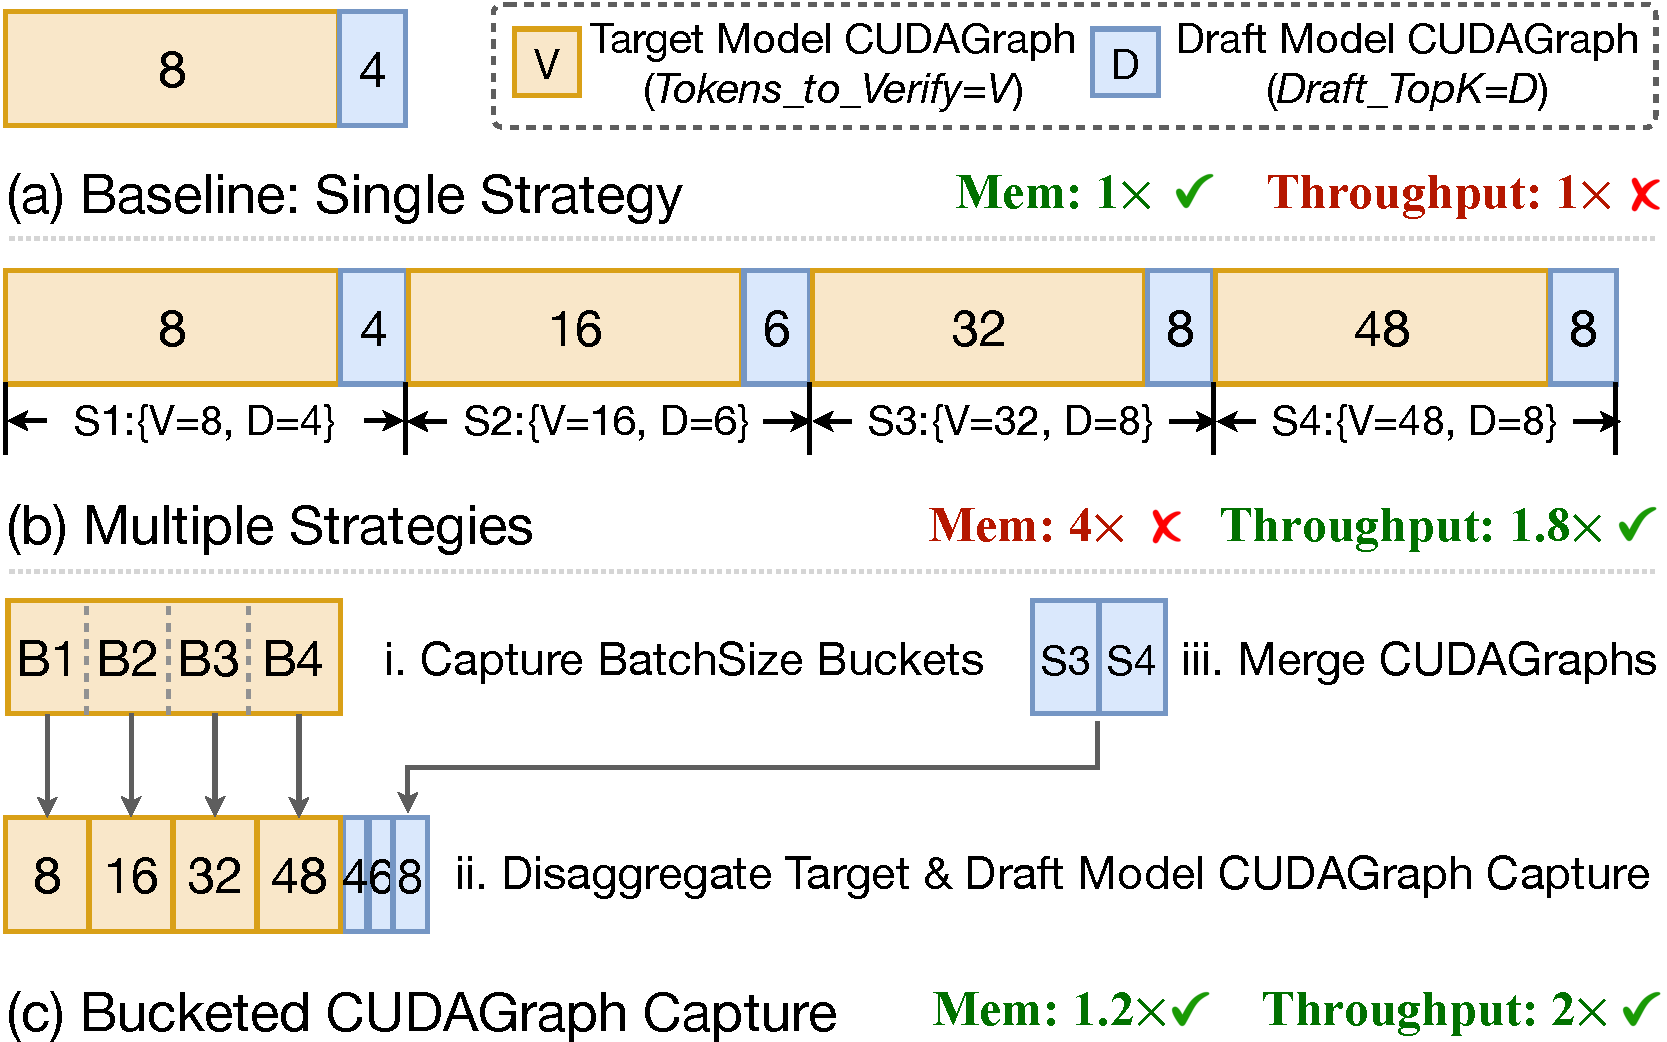
\includegraphics[width=\linewidth]{figures/method/mab.pdf}
  \caption{\textbf{SD 的 CUDA Graph 显存占用。}S1--S4 表示不同 SD 策略，B1--B4 表示批大小桶；图中显存与吞吐数值仅作示意。}
  \label{fig:mab}
\end{figure}

\subsection{自适应 SD 管理器}

\noindent\textbf{树式草拟。}
线性草拟只处理单一序列；树式草拟则扩展这种单分支范式，并行探索多条推测路径。遵循已有方法~\cite{SpecInfer,Eagle2}，我们根据草稿模型的置信度分数（token 概率）构建候选树，如图~\ref{fig:tree} 所示。系统从输入提示“Climate”开始，由草稿模型预测潜在的后续 token。树式方法在每一步探索概率最高的 \texttt{topK} 个选项，例如 \texttt{topK=2} 会得到“change”和“control”；分支过程持续 \texttt{Draft\_Depth} 步，形成候选序列树。最后，系统在树中选择置信度最高的 $\texttt{Tokens\_to\_Verify}=8$ 个 token，并提交给目标模型并行验证。通过同时探索和验证多条潜在序列，树式草拟显著增加了每次验证可接受的 token 数，从而提高整体生成吞吐和 GPU 利用率。

\noindent\textbf{自适应不可或缺。}
SD 虽主要用于加速长尾阶段，我们观察到它在中等批大小下也能带来加速（表~\ref{tab:sd-bs}）。不过，这要求系统根据解码批大小和工作负载特征自适应调整 SD 策略。既有工作~\cite{Eagle1,Eagle2,HASS}主要关注批大小为 1 的场景，限制了真实应用范围。

RL rollout 天然具有高度动态的批大小：开始时批量很大，随后短响应不断完成，批大小迅速缩小。因此，静态 SD 策略既低效又不安全，在大批量下可能触发显存不足（OOM）。自适应 SD 管理器持续调节 SD 参数：选择安全策略以避免 OOM，针对每类工作负载学习有效策略以最大化吞吐，并权衡推测收益与计算开销。此外，对于 SD 收益很小的大批量，它采用弹性机制，只在剩余请求数低于可配置阈值时启用 SD，默认阈值为 32。

\noindent\textbf{显存高效的 CUDAGraph 捕获。}
CUDAGraph 常用于加速 LLM 解码：它记录 CUDA 操作，再以一个整体回放，从而减少推理期间每个 kernel 的启动成本并带来显著加速。但 CUDAGraph 要求为每种批大小和策略分别捕获静态图，其中同时包含目标模型与草稿模型。这种不灵活的范式造成可观的显存占用。在多策略设置下（图~\ref{fig:mab}(b)），显存用量随策略数线性增长，导致模型权重和 KV cache 空间不足，在实践中无法接受。

为了在不付出过高显存成本的情况下容纳更多 SD 策略，我们提出分桶 CUDAGraph 捕获（图~\ref{fig:mab}(c)），包含三项关键优化：（1）\emph{批大小分桶}。系统不为每个可能的批大小捕获静态图，而是利用策略特征，例如大批量通常应验证更少 token，把批大小划分到若干桶（如 B1--B4）。（2）\emph{分别捕获目标模型与草稿模型}。部分配置只影响其中一个模型，例如 \texttt{topK} 只影响草稿器，而 \texttt{Tokens\_to\_Verify} 只影响目标模型，因此分别捕获两类图，避免显存乘法式增长。（3）\emph{跨策略合并捕获}。当不同策略共享相同参数设置时，系统把相应批大小桶合并到同一捕获图中，消除冗余显存开销。

这些优化大幅降低 CUDAGraph 显存占用（表~\ref{tab:cg-mem}），同时提高 rollout 吞吐。吞吐提升来自利用先验知识，不再评测明显不适合特定批大小的次优策略。

\begin{algorithm}[t]
\small
\caption{分桶 $\epsilon$-贪心（BEG）MAB 选择器}
\label{alg:beg}
\begin{algorithmic}[1]
\Require 策略集 $\mathcal S$，批量阈值 $\mathcal T=\{t_1,\ldots,t_m\}$，探索率 $\epsilon$，窗口大小 $w$
\Ensure 选定策略 $s^*$
\State 按 \texttt{Tokens\_to\_Verify} 对 $\mathcal S$ 分组为 $\{\mathcal S_1,\ldots,\mathcal S_m\}$，并按降序排列
\State 定义桶 $\mathcal B_i=[t_i,t_{i+1}-1]$（$i<m$）及 $\mathcal B_m=[t_m,\infty)$
\State 将桶 $\mathcal B_i$ 映射到组 $\mathcal S_i$
\ForAll{$s\in\mathcal S$}
  \State 初始化长度为 $w$ 的双端队列 $R_s,A_s$
\EndFor
\Statex \textbf{记录}（\texttt{elapsed\_time}, \texttt{accept\_lens}, \texttt{batch\_size}）
\State $\bar a\gets(\sum\texttt{accept\_lens})/\texttt{batch\_size}+1$
\State $r_s\gets\bar a\times\texttt{batch\_size}/\texttt{elapsed\_time}$
\State 将 $r_s$ 追加到 $R_s$，将 $\bar a$ 追加到 $A_s$
\Statex \textbf{选择策略}（\texttt{batch\_size}）
\State $V\gets\{s\in\mathcal S_i\mid\texttt{batch\_size}\in\mathcal B_i\}$
\If{$|V|=1$} \State \Return $V$ 中唯一策略 \EndIf
\State 采样 $u\sim\mathrm{Uniform}(0,1)$
\If{$u<\epsilon$}
  \State \Return 从 $V$ 中随机选取的策略 \Comment{探索}
\Else
  \State \Return $\arg\max_{s\in V}\operatorname{Median}(R_s)$ \Comment{利用}
\EndIf
\end{algorithmic}
\end{algorithm}

\subsection{自动调优算法}

\noindent\textbf{分桶 $\epsilon$-贪心 MAB。}
多臂老虎机（MAB）算法是在线决策的经典框架，擅长在动作（“臂”）回报不确定时选择动作并最大化累计收益~\cite{MABResourceAllocation,MAB}。每只“臂”对应一个推测解码配置三元组 $(\texttt{Draft\_Depth},\texttt{topK},\texttt{Tokens\_to\_Verify})$，“回报”反映该生成步骤的效率，即 $\text{accepted\_token\_num}/\text{step\_latency}$。

为自动选择 SD 策略，我们设计了新的在线调优算法——分桶 $\epsilon$-贪心（BEG）MAB 选择器（算法~\ref{alg:beg}）。BEG 采用针对推测解码工作负载定制的 $\epsilon$-贪心策略。它按 \texttt{Tokens\_to\_Verify} 对策略分桶，并动态匹配批大小范围。具体来说，策略集 $\mathcal S$ 按该参数分为 $\{\mathcal S_1,\ldots,\mathcal S_m\}$，每组映射到批大小桶 $\mathcal B_i$。rollout 期间，当前批大小决定相关候选集 $V$。若 $|V|=1$，策略固定；否则 BEG 在探索与利用间选择：以概率 $\epsilon$ 从 $V$ 中均匀随机选择策略进行探索；以概率 $1-\epsilon$ 选择在大小为 $w$ 的滑动窗口内具有最高回报中位数的策略进行利用。算法中的回报同时权衡接受率和延迟成本。维护近期回报的双端队列，使系统能适应 RL 训练期间的非平稳动态。

通过组合分桶策略选择、轻量 $\epsilon$-贪心探索和滑动窗口回报估计，BEG 在适应工作负载变化的同时，减少穷举探索的开销。因此，\SysName 能跨多种批大小与推测解码策略扩展，无需手工调优。

\subsection{无模型草稿器}

\noindent\textbf{利用 rollout 间的相似性。}
在 RL rollout 阶段，针对同一提示生成的候选响应往往有明显的\emph{序列相似性}和重复模式，例如常见数学记号或代码语法结构。这说明，频繁出现的短程 token 依赖可以通过检索方法有效预测。为利用这一点，\SysName 在主要的学习型草稿器之外，加入互补的非参数草拟策略。该无模型草稿器根据每个提示对应的 rollout 响应，动态构建 n-gram 检索数据库；它以紧邻上下文，即前序 n-gram 为条件查询数据库，高效预测常见的后续 token 序列。

在 \SysName 中，无模型草稿器既是稳健基线，也是不可或缺的后备机制。当学习型草稿器不可用（如训练初期）或预计效率较低时，策略选择器会动态启用基于检索的草稿器。这种双草稿器方法确保推测解码加速贯穿 RL 全流程，持续带来效率收益。

\section{评测}
\label{sec:evaluation}

\begin{figure*}[t]
  \centering
  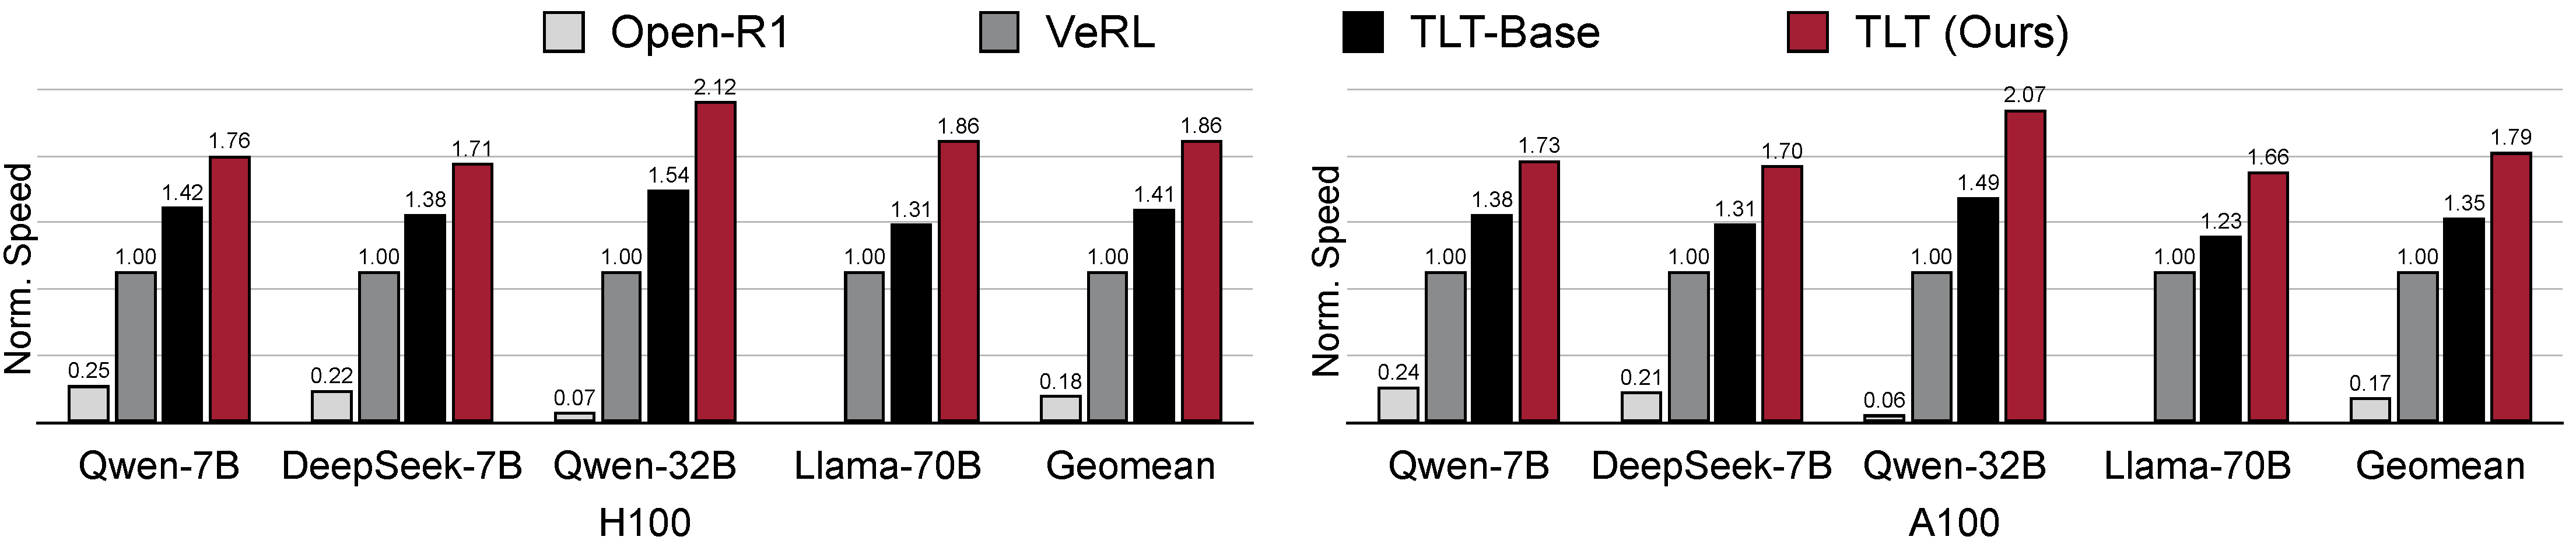
\includegraphics[width=\textwidth]{figures/results/main_speed.pdf}
  \caption{\textbf{端到端训练速度评测。}纵轴表示各系统运行 GRPO~\cite{DeepSeekMath}时的相对训练吞吐。\SysName 相比最先进的 RL 训练系统 VeRL~\cite{HybridFlow}实现 $1.7$--$2.1\times$ 加速。}
  \label{fig:main-speed}
\end{figure*}

\begin{figure*}[t]
  \centering
  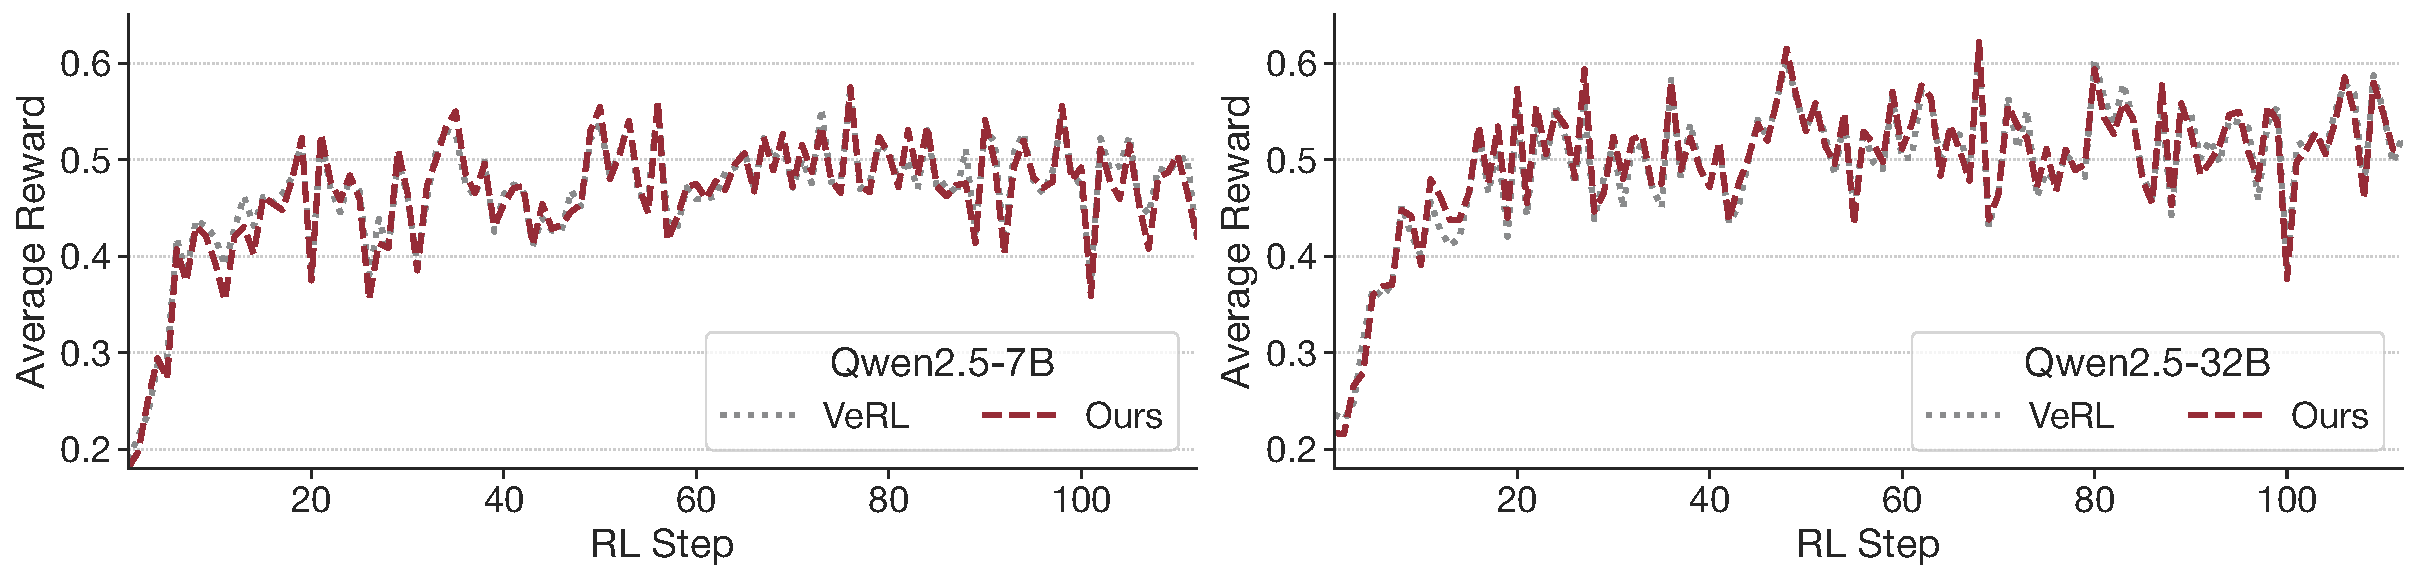
\includegraphics[width=\textwidth]{figures/results/rl_trace.pdf}
  \caption{\textbf{端到端训练曲线。}VeRL 与 \SysName 使用 Qwen2.5-7B 和 Qwen2.5-32B 时的平均奖励曲线。}
  \label{fig:rl-trace}
\end{figure*}

\subsection{实验设置}

\noindent\textbf{实现。}
我们在 VeRL~\cite{HybridFlow}之上实现 \SysName，并使用 Ray~\cite{Ray}进行分布式执行。Worker Coordinator 由使用 ZeroMQ~\cite{ZeroMQ}消息传递的集中式控制器实现。自适应草稿器基于 EAGLE 的训练管线实现，并使用 FSDP2~\cite{FSDP2}训练；异步检查点采用 PyTorch DCP~\cite{DCP}。为进一步提高生成效率，我们使用 SGLang~\cite{SGLang}作为 rollout 后端，并按照相关实现~\cite{SGLangMAB}加入 SD 的自适应启用、草稿器权重更新和 BEG-MAB 调优器。此外，我们采用已有方法~\cite{LookaheadKDD}作为无模型草稿器。

\noindent\textbf{测试平台。}
我们在由 8 台 NVIDIA DGX H100~\cite{dgx-h100}服务器组成的集群上实验，共 64 张 GPU。每台服务器配有 8 张 NVIDIA H100 GPU、两颗 Intel Xeon Platinum 8480C CPU（共 112 核）以及 2TB 内存。GPU 之间通过 900GB/s NVLink 互连，节点间通过 NVIDIA Mellanox 400Gb/s InfiniBand 通信。为评估系统跨异构硬件的性能，我们还在配有 NVIDIA DGX A100 服务器的另一个集群上实验。除非另有说明，默认实验均在 H100 GPU 上进行。

\noindent\textbf{模型。}
遵循 DeepSeek-R1~\cite{DeepSeekR1}介绍的训练流程，推理 RL 既可从微调模型开始，也可直接从未经额外微调的基础模型开始。为证明 \SysName 能稳健适配不同模型架构、规模与训练范式，我们评测以下模型：
\begin{enumerate}[label=(\arabic*),topsep=2pt,itemsep=1pt,leftmargin=20pt]
  \item \emph{Qwen2.5-7B}（Qwen2.5-7B）：常用基础模型；
  \item \emph{DeepSeek-R1-Distill-Qwen-7B}（DeepSeek-7B）：具备良好初始推理能力的蒸馏模型；
  \item \emph{Qwen2.5-32B}（Qwen-32B）：与 DAPO~\cite{DAPO}相同，未经额外微调的较大基础模型；
  \item \emph{Llama-3.3-70B-Instruct}（Llama-70B）：用于评估可扩展性的较大指令微调模型。
\end{enumerate}

\noindent\textbf{数据集。}
主要 RL 训练数据集使用 Eurus-2-RL~\cite{Prime}的一个子集；这是为推理 RL 精心整理的综合数据集，包含配有验证器的数学与编程题，验证器分别是 LaTeX 答案和测试用例。编程题来自 CodeContests~\cite{CodeContests}、Codeforces~\cite{codeforces}等竞赛编程来源，数学题难度则从高中到奥林匹克竞赛级别~\cite{numina_math}。草稿器训练使用 OpenThoughts2-1M~\cite{OpenThoughts2-1M}的一个子集进行预热。

\noindent\textbf{RL 设置。}
我们主要遵循 DeepSeek 提出的推理 RL 算法 GRPO~\cite{DeepSeekR1,DeepSeekMath}。具体而言，每个提示的温度设为 0.9，最大生成长度设为 32K token，与常见 RL 训练设置一致。rollout 引擎根据模型规模采用 TP=2、4 或 8。全部实验都使用 Adam 优化器~\cite{Adam}进行混合精度训练，并采用 BF16 精度。

\noindent\textbf{基线。}
我们考虑以下基线：
\begin{enumerate}[label=(\arabic*),topsep=2pt,itemsep=1pt,leftmargin=20pt]
  \item \emph{Open-R1}~\cite{openr1}：建立在 TRL~\cite{TRL}之上的常用 RL 训练框架，集成 vLLM~\cite{vLLM}执行 rollout，集成 DeepSpeed~\cite{ZeRO}执行训练。目前它只支持模型分离放置，要求服务和训练在不同节点执行。
  \item \emph{VeRL}~\cite{HybridFlow}：ByteDance 开源的最先进 RL 训练框架，通过 GPU 分时复用，使模型能够共置于共享设备。
  \item \emph{\SysName-Base}：支持普通推测解码的基础实现；具体而言，关闭自适应草稿模型，改用无模型草稿器。
\end{enumerate}

\noindent\textbf{指标。}
遵循 VeRL~\cite{HybridFlow}，端到端评测使用 token 吞吐（token/s）。计算方法是：用一个全局批中提示与响应的 token 总数，除以单个 RL 步骤的持续时间。我们先执行一个预热步骤，随后对三个训练步骤取平均，并使用已经训练好的草稿模型评测。

\subsection{端到端评测}

我们在多种 GPU 平台（NVIDIA H100 和 A100）与多种 LLM 规模下，将 \SysName 和 Open-R1~\cite{openr1}、VeRL~\cite{HybridFlow}等常用 RL 训练框架比较。图~\ref{fig:main-speed} 表明，\SysName 始终优于 VeRL。Open-R1 的表现始终较差，主要原因是它难以并发充分利用全部 GPU，且 rollout 批大小与训练批大小耦合过紧。A100 平台也观察到相似的显著收益，说明该方法跨硬件世代有效。我们还报告了 \SysName-Base 的结果；它采用无模型草稿器，同样取得良好收益，说明 \SysName 框架能在整个训练过程中持续提升效率。这些端到端收益直接来自 \SysName 对推理 RL 长尾 rollout 瓶颈的缓解。

此外，图~\ref{fig:rl-trace} 展示了 VeRL 和 \SysName 使用 Qwen2.5-7B 与 Qwen2.5-32B 进行 RL 训练时的平均奖励曲线。两条曲线高度重合，表明 \SysName 保持了模型质量；这也证实，自适应草稿模型和 rollout 引擎可以加速训练，而不损害底层 RL 算法的学习动态。

\subsection{自适应 SD 评测}

\begin{figure}[t]
  \centering
  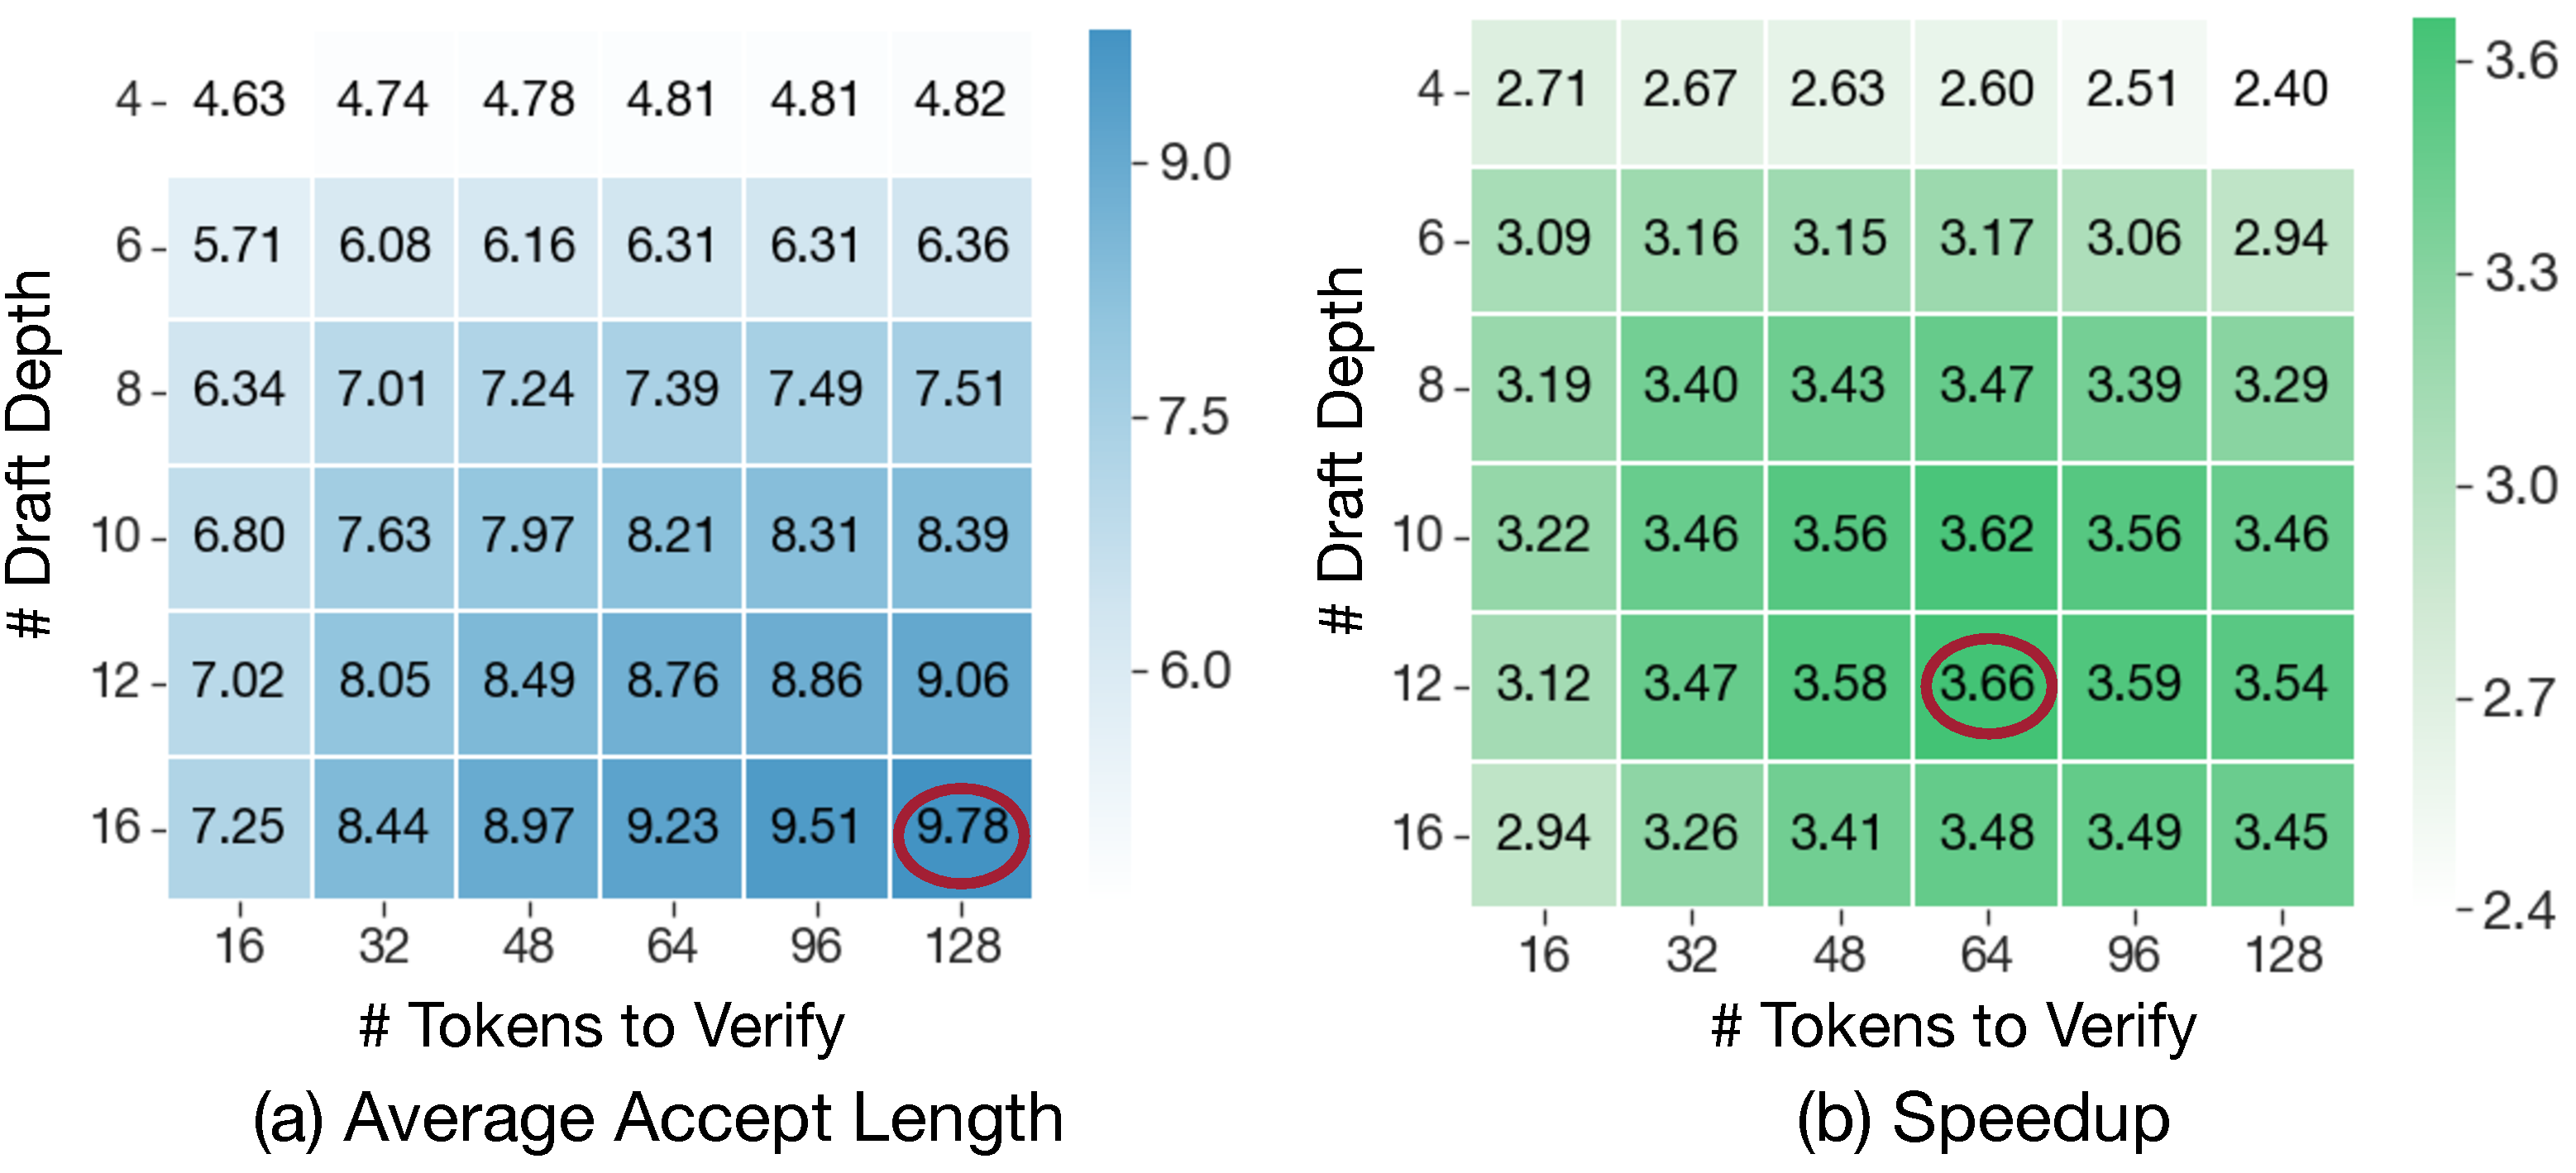
\includegraphics[width=\linewidth]{figures/results/sd_heatmap.pdf}
  \caption{\textbf{推测解码超参数的影响。}使用 Qwen-32B（TP=4）测量。}
  \label{fig:sd-heatmap}
\end{figure}

\noindent\textbf{自适应 SD 策略的作用。}
调节 SD 配置对取得最优加速至关重要。图~\ref{fig:sd-heatmap} 展示了在批大小为 1、\texttt{topK=8}且启用 CUDA Graph 时，\texttt{Draft\_Depth} 和 \texttt{Tokens\_to\_Verify} 如何影响推测解码性能。为了在网格搜索中获得更稳定的接受长度，温度设为 0。增加草稿深度通常会提高平均接受长度（a），但当深度足够大后，收益逐渐饱和；（b）给出相对非推测基线的加速比。这说明，只最大化接受长度并不够；草拟参数必须针对实际性能而不是中间指标进行调优。

对于 \texttt{topK}，我们发现草拟效率对其取值相对不敏感（表~\ref{tab:topk}）。为兼顾整体效率和框架简洁性，我们在 MAB 自动调优器中固定该超参数。

\begin{table}[t]
\centering\small
\caption{\textbf{\texttt{topK} 对推测解码的影响。}Qwen-32B，H100（TP=4），\texttt{Draft\_Depth=12}、\texttt{Tokens\_to\_Verify=64}。}
\label{tab:topk}
\resizebox{\linewidth}{!}{
\begin{tabular}{lcccccc}
\toprule
TopK & 4 & 6 & 8 & 10 & 12 & 16 \\
\midrule
接受长度 & 8.29 & 8.66 & 8.67 & 8.67 & 8.60 & 8.42 \\
加速比 & 3.51$\times$ & \textbf{3.65}$\times$ & 3.64$\times$ & 3.64$\times$ & 3.56$\times$ & 3.47$\times$ \\
\bottomrule
\end{tabular}}
\end{table}

推测解码的最优配置也随输入批大小而变化（表~\ref{tab:sd-bs}）。尽管加速比随批大小增长而下降，模型在批大小为 32 时仍能从 SD 获得可观收益。另一个关键观察是，\texttt{Tokens\_to\_Verify} 应随批大小调整：批量越大，验证较少 token 时性能越优。这些结果进一步证明，BEG MAB 选择器能够在运行请求数动态变化时识别合适配置。

\noindent\textbf{自适应 SD 案例研究。}
图~\ref{fig:rollout-profile} 给出了一个 RL 步骤的 rollout 剖析案例：在 H100 GPU 上用 Qwen-32B 处理 128 个请求。若从始至终应用 SD，在活跃请求较多的早期阶段可能反而变慢。\SysName 只在剩余请求数低于阈值（默认为 32）且 SD 开始有益时切换到 SD。在启用 SD 的区间内，系统还根据当前请求数动态适配 SD 配置以最大化吞吐。总体而言，\SysName 相比不使用推测解码的基线系统实现 $2.44\times$ 加速。

\noindent\textbf{GPU 多样性与可扩展性。}
我们在多种 GPU 架构和集群规模上评测 \SysName。如表~\ref{tab:gpu} 所示，\SysName 在数据中心 GPU 和消费级 GPU 上均获得稳定加速。端到端训练结果（表~\ref{tab:scale}）进一步表明，随着模型和集群规模增长，\SysName 的加速更加明显，显示出对大规模推理 RL 训练的良好可扩展性。

\begin{table}[t]
\centering\small
\caption{\textbf{不同 GPU 类型上的 rollout 吞吐（token/s）与加速。}Qwen2.5-7B，BS=1，TP=1。}
\label{tab:gpu}
\begin{tabular}{lrrc}
\toprule
GPU & 使用 SD & 不使用 SD & 加速比 \\
\midrule
B200 & 605.05 & 259.71 & 2.33$\times$ \\
H100 & 430.24 & 164.65 & 2.61$\times$ \\
A100 & 259.01 & 92.83 & 2.79$\times$ \\
RTX 5090 & 293.84 & 100.89 & 2.91$\times$ \\
RTX 4090 & 187.44 & 65.28 & 2.87$\times$ \\
RTX 3090 & 166.41 & 51.75 & 3.22$\times$ \\
\bottomrule
\end{tabular}
\end{table}

\begin{table}[t]
\centering\small
\caption{\textbf{不同 GPU 规模下的端到端训练加速。}}
\label{tab:scale}
\resizebox{\linewidth}{!}{
\begin{tabular}{lcccc}
\toprule
节点数（8 GPU/节点） & 1 & 2 & 4 & 8 \\
\midrule
Qwen2.5-7B & 1.21$\times$ & 1.45$\times$ & 1.62$\times$ & 1.76$\times$ \\
Qwen2.5-32B & OOM & OOM & 1.83$\times$ & 2.12$\times$ \\
\bottomrule
\end{tabular}}
\end{table}

\noindent\textbf{分桶 CUDAGraph 捕获。}
为多个 SD 策略准备 CUDAGraph 可能消耗大量显存。如表~\ref{tab:cg-mem} 所示，若为四个候选策略分别朴素捕获图，显存用量会从 7.81GB 增至 30.39GB。分桶 CUDAGraph 把图显存降至 10.69GB，相比朴素方法减少 $2.8\times$，且只比单一静态策略略高，使自适应调优器能灵活切换 SD 配置并最大化效率。

\begin{table}[t]
\centering\small
\caption{\textbf{批大小对推测解码的影响。}Qwen-32B，H100（TP=4），\texttt{Draft\_Depth=10}、\texttt{topK=8}。}
\label{tab:sd-bs}
\resizebox{\linewidth}{!}{
\begin{tabular}{lcccc}
\toprule
& \multicolumn{4}{c}{验证 token 数} \\
\cmidrule(lr){2-5}
批大小 & 16 & 32 & 48 & 64 \\
\midrule
1 & 3.22$\times$ & 3.46$\times$ & 3.56$\times$ & \textbf{3.62}$\times$ \\
2 & 3.08$\times$ & 3.28$\times$ & \textbf{3.39}$\times$ & 3.38$\times$ \\
4 & 3.01$\times$ & 3.09$\times$ & \textbf{3.13}$\times$ & 2.98$\times$ \\
8 & \textbf{2.73}$\times$ & 2.63$\times$ & 2.51$\times$ & 2.27$\times$ \\
16 & \textbf{2.67}$\times$ & 2.52$\times$ & 2.24$\times$ & 1.91$\times$ \\
32 & \textbf{2.48}$\times$ & 2.23$\times$ & 1.90$\times$ & 1.70$\times$ \\
\bottomrule
\end{tabular}}
\end{table}

\begin{figure}[t]
  \centering
  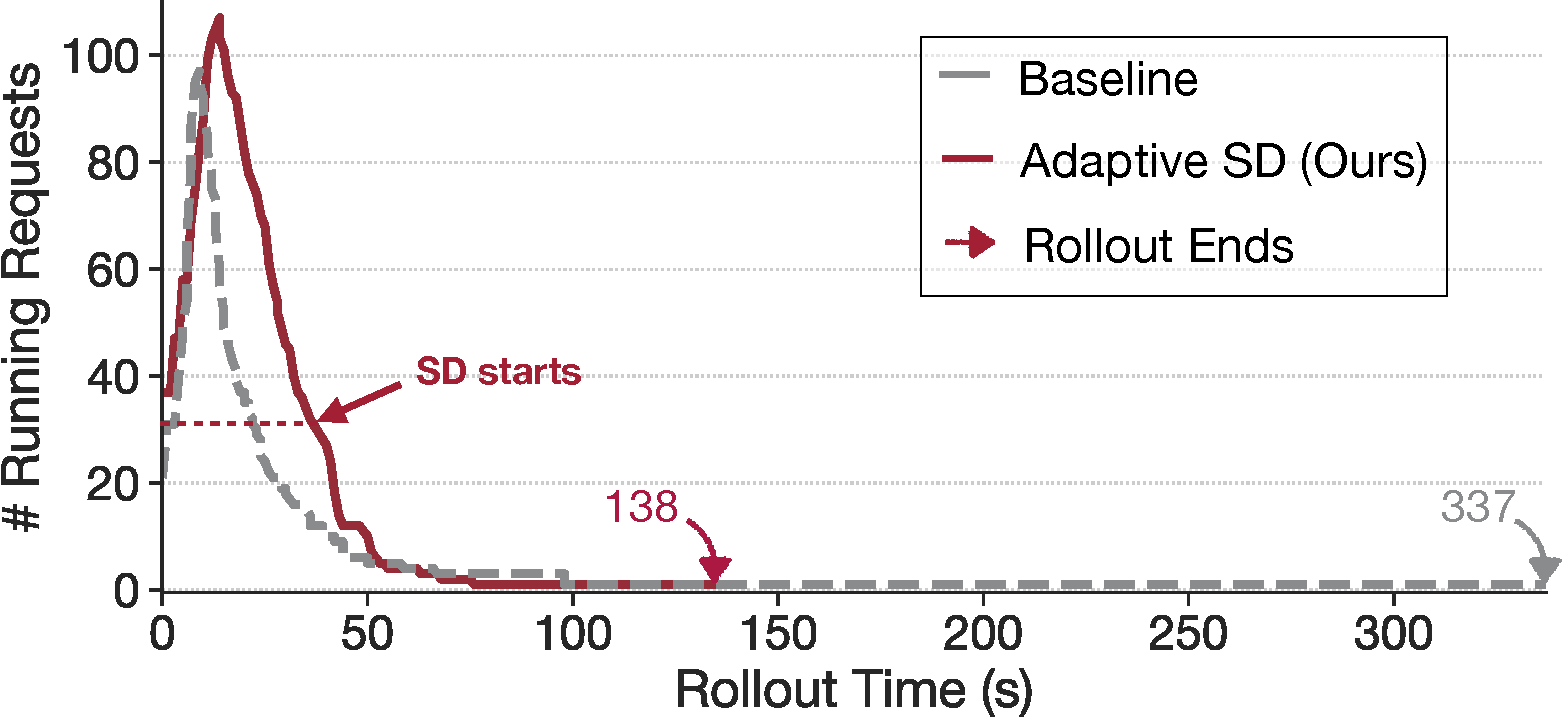
\includegraphics[width=.9\linewidth]{figures/results/rollout_profile.pdf}
  \caption{\textbf{rollout 运行请求数剖析。}使用 Qwen-32B（TP=4）时，以自适应解码和普通解码处理 128 个请求的示例。}
  \label{fig:rollout-profile}
\end{figure}

\subsection{Spot Trainer 评测}

\noindent\textbf{训练自适应草稿器。}
图~\ref{fig:training-curve} 给出一条训练曲线示例，展示自适应草稿器的训练过程。初始预热后，草稿器的 top-3 下一 token 预测准确率显著提高。在一个 RL 步骤后更新目标模型时，权重更新导致分布偏移，草稿器准确率会暂时下降；但只需随后几次草稿器训练迭代，准确率便能迅速恢复，证明了自适应方法的有效性和稳健性。

\noindent\textbf{自适应草稿器的有效性。}
表~\ref{tab:adaptive} 展示了自适应训练草稿模型的效果。借助该机制，\SysName 在 RL 训练任务和下游评测中，都能为 Target-R 模型稳定取得更长的平均接受长度，说明对齐与性能得到改善。

\begin{table}[t]
\centering\small
\caption{\textbf{分桶 CUDAGraph 降低显存占用。}Llama-3-8B，H100（TP=4），搜索空间含 4 个策略。}
\label{tab:cg-mem}
\begin{tabular}{lc}
\toprule
方法 & 显存占用 \\
\midrule
单一策略 & 7.81 GB \\
普通多策略 & 30.39 GB \\
分桶 CUDAGraph & 10.69 GB \\
\bottomrule
\end{tabular}
\end{table}

图~\ref{fig:accept-rate} 进一步印证了这一点：它展示草拟序列中不同 token 位置的接受概率。由于目标模型输出分布发生变化且误差不断累积，普通草稿模型很难准确预测较远位置的 token，从而严重限制有效接受长度。自适应草稿器则能在这些位置维持更高的接受概率，说明它可以缓解目标模型演化的影响，并保持更长的接受长度。

\noindent\textbf{高效 Spot Trainer。}
Spot Trainer 实现了可抢占、高吞吐的训练，运行时开销可忽略不计。在其优化中，选择性异步检查点（图~\ref{fig:spot-optim}(a)）使训练器可被抢占，且不会造成显著工作损失。相比普通同步设计，我们把保存过程卸载到后台线程，并只选择性转储草稿模型的可训练参数，从而把检查点延迟降低 $9.2\times$。图~\ref{fig:spot-optim}(b) 展示序列打包的效果：它连接变长序列，消除 padding token 上的无效计算，相比普通 batching 将训练吞吐提高 $2.2\times$。

\begin{figure}[t]
  \centering
  
\includegraphics[width=.9\linewidth]{figures/results/training_curve.pdf}
  \caption{\textbf{自适应训练期间草稿模型的准确率。}自适应草稿器的 top-3 准确率持续上升；目标模型更新虽造成小幅下降，草稿器会迅速适应并恢复。}
  \label{fig:training-curve}
\end{figure}

\begin{table}[t]
\centering\small
\caption{\textbf{自适应草稿器的有效性。}Target-Base 表示 Qwen2.5-7B，Target-R 表示 RL 后的模型；下游任务包括 MTBench~\cite{Arena}中的数学、编程和推理领域。}
\label{tab:adaptive}
\resizebox{\linewidth}{!}{
\begin{tabular}{lcccc}
\toprule
& \multicolumn{2}{c}{RL 训练} & \multicolumn{2}{c}{下游任务} \\
\cmidrule(lr){2-3}\cmidrule(lr){4-5}
& Target-Base & Target-R & Target-Base & Target-R \\
\midrule
接受长度 & 4.59 & 6.53 & 3.76 & 5.15 \\
\bottomrule
\end{tabular}}
\end{table}

\begin{figure}[t]
  \centering
  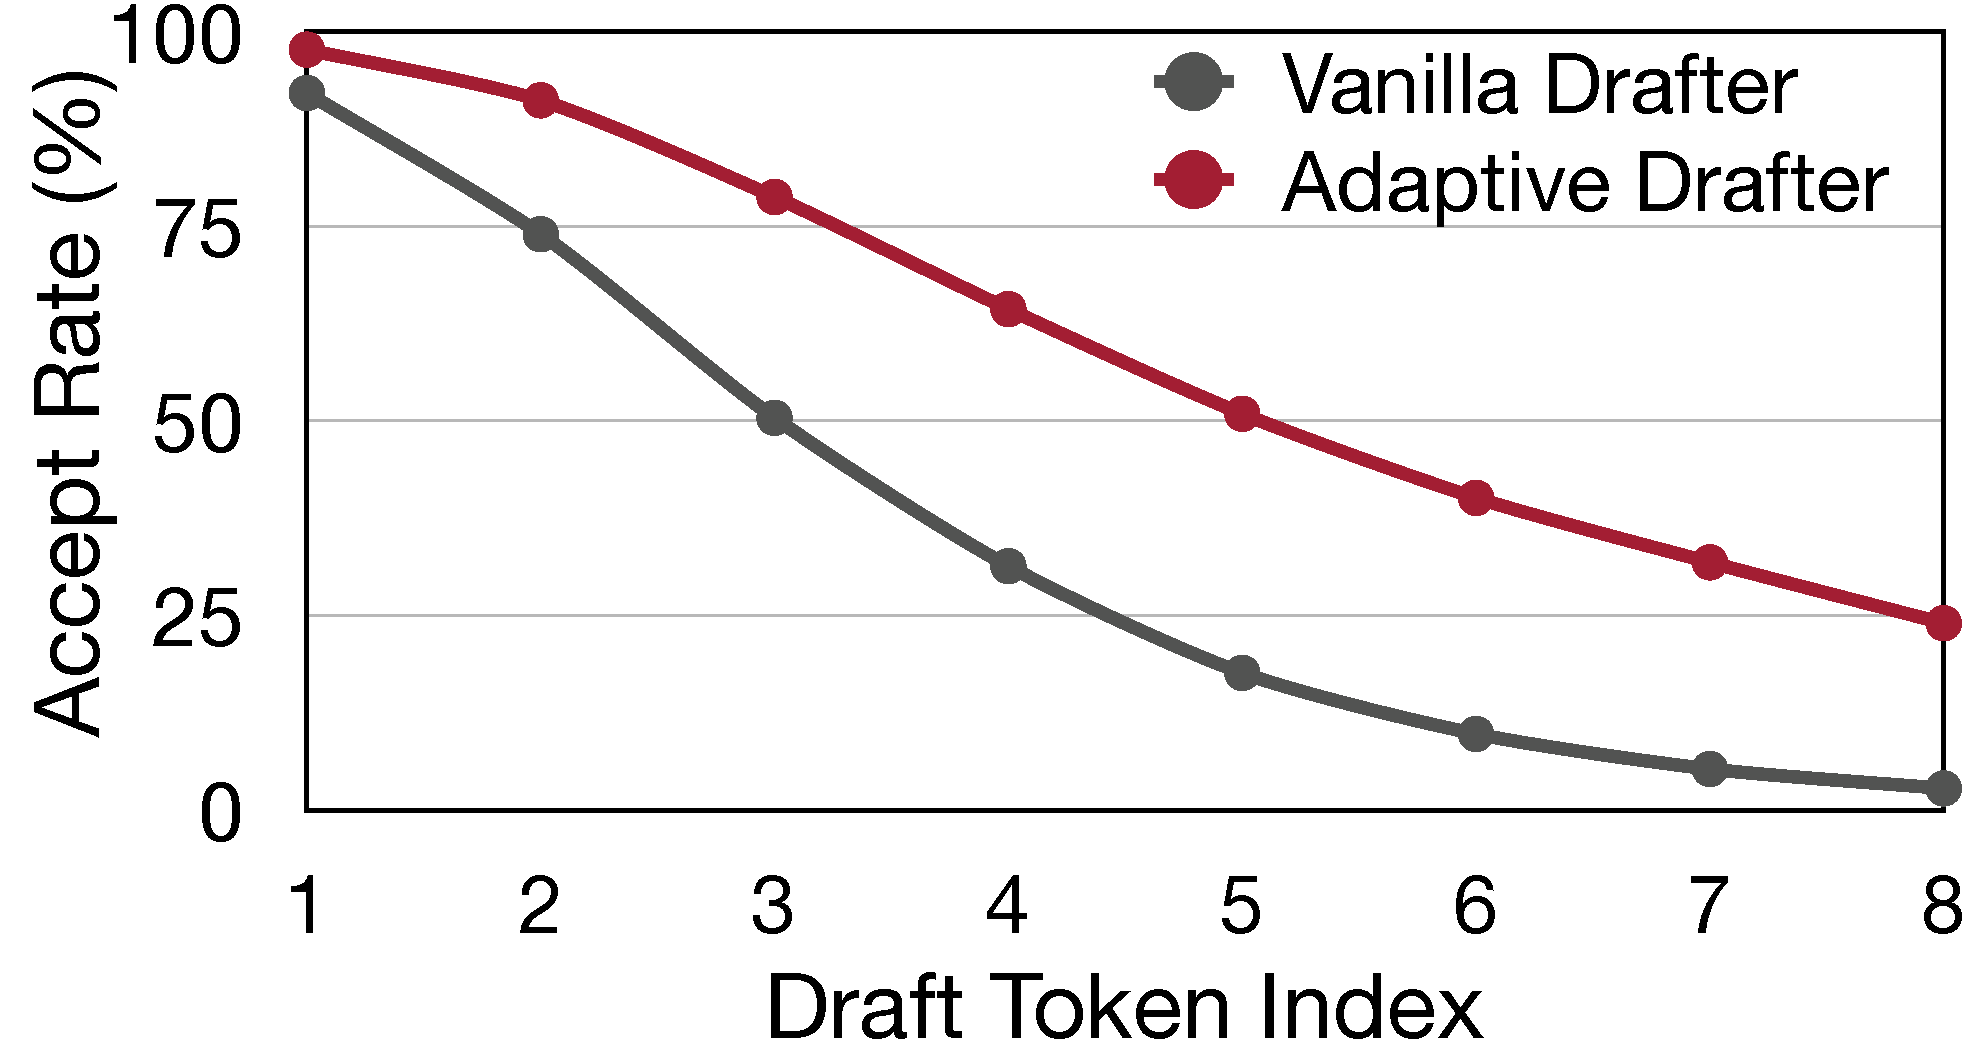
\includegraphics[width=.75\linewidth]{figures/results/alpha_ablate.pdf}
  \caption{\textbf{不同草稿模型的 token 接受率。}在 rollout 场景中，我们的自适应草稿模型预测较远 token 时取得明显更高的接受率。}
  \label{fig:accept-rate}
\end{figure}

\noindent\textbf{系统开销分析。}
我们识别出 \SysName 的三项主要开销：（1）阶段转换开销。与 VeRL~\cite{HybridFlow}相比，额外的草稿器权重更新和优化器卸载会引入开销；但由于草稿模型小得多，这部分少于 RL 步骤时间的 $1\%$。（2）SD 切换开销。从普通解码切换到 SD 时，草稿模型在大批量阶段最初未激活，因此需要重新预填充来启用 SD，耗时不超过 3 秒。（3）草稿器训练协调开销。Spot Trainer 执行时偶发竞争会带来开销；不过，草稿器无需每个 RL 步骤都训练，每 10 步训练一次已足以维持准确率。总体而言，\SysName 的性能收益远大于这些开销，最终带来端到端加速。

\subsection{草稿器架构分析}

为证明 \SysName 框架的通用性，我们集成并评测了多种最先进推测解码方法，结果见表~\ref{tab:drafters}。HASS~\cite{HASS}和 Eagle-3~\cite{Eagle3}等较新的 SD 方法虽能取得略高的接受长度和吞吐，其“训练时测试”技术却需要在训练期间进行多次前向传播，显著增加单步训练开销和模型收敛难度。由于 rollout 气泡内的时间预算有限，我们选择 Eagle~\cite{Eagle2}，因为它性能相近且更简洁。

\begin{table}[t]
\centering\small
\caption{\SysName 中不同 SD 方法的比较。Qwen2.5-7B，TP=2，BS=1，H100；训练成本归一化为 Eagle 单步成本。}
\label{tab:drafters}
\resizebox{\linewidth}{!}{
\begin{tabular}{lcccc}
\toprule
方法 & 接受长度 & 吞吐 & 加速比 & 训练成本 \\
\midrule
基线（无 SD） & 1.00 & 242.11 & 1.00$\times$ & -- \\
HASS~\cite{HASS} & 6.67 & 553.91 & 2.29$\times$ & 3$\times$ \\
Eagle-3~\cite{Eagle3} & 6.83 & 617.42 & 2.55$\times$ & 7$\times$ \\
Eagle~\cite{Eagle2} & 6.53 & 542.12 & 2.24$\times$ & 1$\times$ \\
\bottomrule
\end{tabular}}
\end{table}

\subsection{在线推测解码（OSD）讨论}

OSD~\cite{OSD}使用广义知识蒸馏（GKD）训练草稿模型，使其在在线服务的分布变化下保持对齐。相比之下，\SysName 关注目标模型权重持续演化的 RL 训练。Eagle 训练已经把知识蒸馏作为损失项，OSD 则进一步探索反向知识蒸馏。我们在表~\ref{tab:osd} 中研究不同训练范式的影响。结果表明，对于通用小模型（如 Qwen-0.5B）以及 \SysName 默认使用的 Eagle 训练方法，OSD 风格训练都比监督微调（SFT）更有效地提高草稿模型质量。

\begin{table}[t]
\centering\scriptsize
\caption{OSD 风格训练对不同草稿模型的影响。Qwen2.5-7B 目标模型，H100，TP=2，BS=1。}
\label{tab:osd}
\resizebox{\linewidth}{!}{
\begin{tabular}{lrrrrrr}
\toprule
草稿模型 & 原始接受长度 & 原始吞吐 & 训练后接受长度 & 训练后吞吐 & +OSD 接受长度 & +OSD 吞吐 \\
\midrule
Qwen2.5-0.5B & 5.95 & 363.87 & 6.68 & 408.51 & 6.89 & 421.35 \\
Eagle & 1.57 & 130.34 & 6.53 & 542.12 & 6.77 & 562.04 \\
\bottomrule
\end{tabular}}
\end{table}

\section{讨论}

\noindent\textbf{更多应用场景。}
本文主要研究如何通过缓解长尾 rollout，以推测解码加速 RL 训练。我们认为，这项技术也为更广泛的应用打开了很有希望的方向。例如：（1）\emph{所有响应都很长}。当所有 rollout 都很长、没有尾部差异时，每个请求都需要大量 KV cache 容量，系统常因此受 KV cache 限制并发生请求驱逐，导致运行批大小受限。这种工作负载自然落入推测解码的“甜点区”，可以加速解码。（2）\emph{包含工具调用 RL 的多轮 rollout}。在包含工具调用的多轮 RL 中，部分请求执行不使用 GPU 的工具，而其 KV cache 仍驻留在 GPU 上。这减少了活跃解码请求数，再次形成有利于本文推测解码方法的运行区间。（3）\emph{在线服务与边缘部署}。当目标模型固定时，可以把 \SysName 训练得到的草稿模型直接部署用于推理。在这些部署场景中，自适应推测解码仍非常有效，尤其适合处理变化的负载。把本文方法扩展到这些场景，是值得期待的未来方向。

\noindent\textbf{能否打破 RL 同步？}
\SysName 的目标是在不修改底层算法 on-policy 要求的前提下提高 RL 训练效率。人们可能会问，能否在漫长的解码阶段使用部分 rollout 异步更新模型，以进一步加速训练。尽管这一方案很有吸引力，却可能改变底层 RL 算法，进而损害收敛和模型性能。采用连续 batching 的异步 RL~\cite{AReaL}通常会在一次 rollout 中混合多个策略版本，可能使梯度估计产生偏差并改变学习动态，例如从 on-policy 漂移为 off-policy。要安全采用这种范式，还需要额外的算法修改。更平衡的做法是允许有限异步，同时保持算法正确性并提高硬件利用率。即使在这种设置下，重尾 rollout 问题依然存在；本文的推测解码可以与有限异步 RL 结合，在\emph{不}引入额外损失或策略陈旧性的情况下进一步加速训练。

\begin{figure}[t]
  \centering
  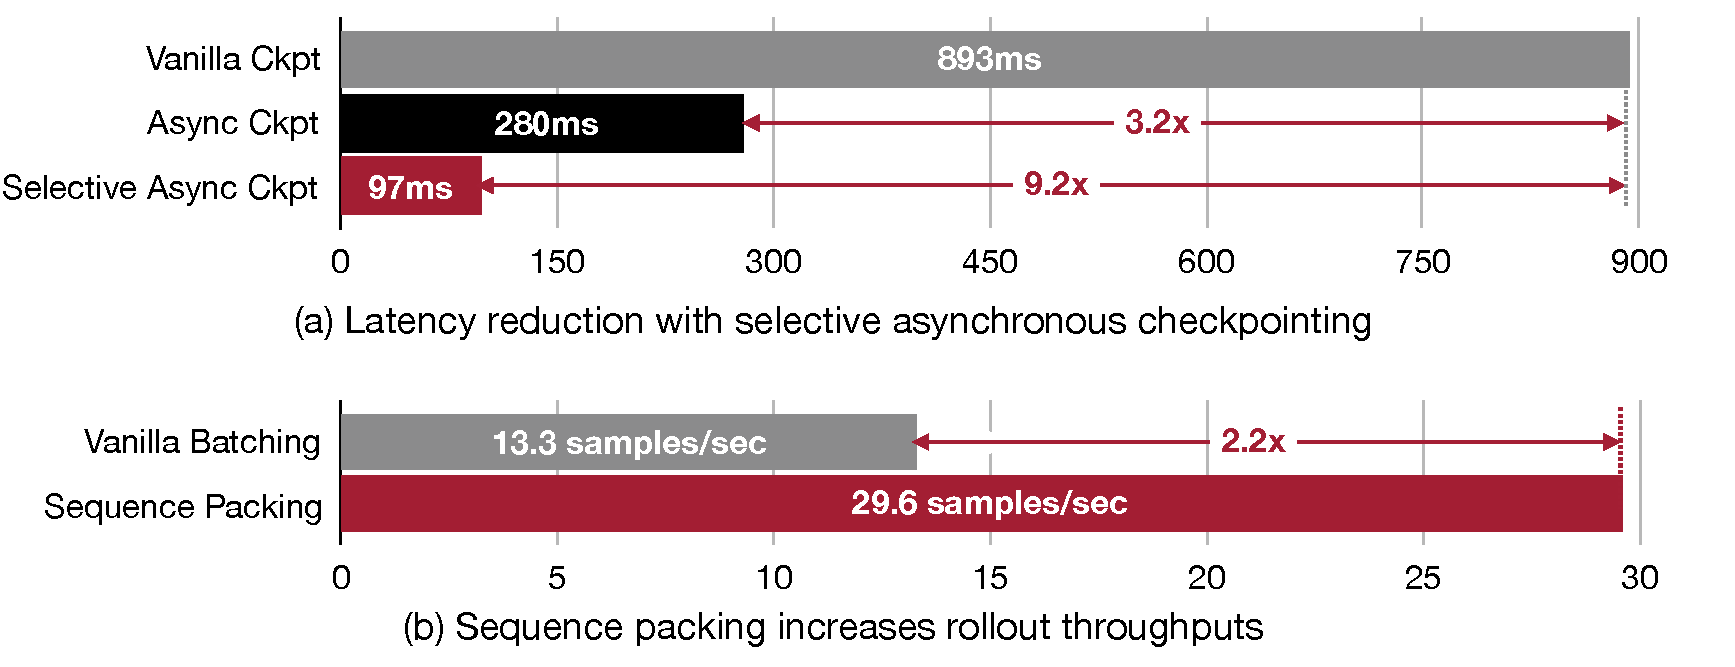
\includegraphics[width=.95\linewidth]{figures/results/spot_trainer.pdf}
  \caption{\textbf{选择性异步检查点与序列打包的效果。}}
  \label{fig:spot-optim}
\end{figure}

\noindent\textbf{\SysName 能否用于其他 RL 算法？}
GRPO 是推理 RL 中广泛使用的算法结构。RLOO~\cite{RLOO}、DAPO~\cite{DAPO}、REINFORCE~\cite{REINFORCE}和 REINFORCE++~\cite{REINFORCEpp}等替代方案通常共享相同的整体训练工作流，主要区别在奖励形式和 KL 正则化的使用方式。这些算法变体与自适应草稿器和 spot 训练设计完全兼容，说明 \SysName 可以直接加速广泛的 RL 方法。

\section{相关工作}

\noindent\textbf{面向 LLM 的 RL 系统。}
已有多个系统试图优化基于人类反馈的强化学习（RLHF）~\cite{InstructGPT}训练管线。DeepSpeed-Chat、GEAR、VeRL、FlexRLHF 和 NeMo-Aligner 等框架~\cite{DeepSpeedChat,GEAR,HybridFlow,FlexRLHF,NeMoAligner}提供可扩展的端到端方案，支持多种对齐算法和并行技术。RLHFuse~\cite{RLHFuse}采用细粒度调度与阶段融合来提高 GPU 利用率；ReaLHF~\cite{ReaLHF}引入动态参数重分配，使 3D 并行策略能灵活适应各个 RLHF 阶段。这些工作主要优化 RLHF 流程固有的多模型管理，却忽视 rollout 阶段的关键性能瓶颈，导致现有系统在推理 RL 任务上效率不足。本文专门优化 rollout 瓶颈，以与既有系统正交的自适应草稿器填补这一空白。近期工作~\cite{AReaL,StreamRL,zhou2025april}尝试通过允许使用陈旧响应更新模型或提前终止 rollout，缓解 RL 的同步约束。RollPacker~\cite{gao2025rollpacker}引入 tail batching；然而，即使查询相同，推理轨迹长度仍可能差异巨大，限制了其效果。这些策略虽能加速训练，却可能降低模型质量。相比之下，本文方法保留原始 RL 算法，在取得显著效率收益的同时保证无损训练。

\noindent\textbf{推测解码。}
推测解码~\cite{SpeculativeDecoding,chen2023accelerating,AdaServe}由目标模型并行验证候选 token，从而增加每一步生成的 token 数并加速 LLM 推理。相关改进覆盖多种策略：检索式方法~\cite{REST,saxena2023PLD,lookahead}无需训练额外草稿模型；另一些方法直接修改目标模型，Medusa 系列~\cite{Medusa}增加多个预测头，Hydra~\cite{Hydra}进一步建模这些预测之间的相关性；SpecInfer~\cite{SpecInfer}则创新性地采用树式推测解码，以扩大候选搜索空间。OSD~\cite{OSD}用知识蒸馏训练草稿模型，使其在在线服务的分布变化下保持对齐。EAGLE~\cite{Eagle1,Eagle2,Eagle3}另外训练紧凑的专用自回归草稿模型；HASS~\cite{HASS}在训练中模拟多步预测，以缓解训练--推理不一致并提高草稿模型准确率。近期工作还把推测思想用于高效推理 LLM：RSD~\cite{RSD}使用奖励模型指导推测，SpecReason~\cite{SpecReason}则用轻量模型推测执行中间推理步骤。不同于这些为静态模型推理设计的方法，本文关注目标模型持续更新的动态训练场景。

\section{结论}

总之，\SysName 通过自适应草稿模型缓解推理 RL 训练的长尾瓶颈，在不损害模型质量的情况下显著提高吞吐。其自适应体现在两个层面：训练期间适应目标模型更新，推理期间适应变化的批大小。因此，系统既提升端到端训练效率，又免费产出可用于后续部署的高质量草稿模型。

\section*{致谢}
衷心感谢论文指导人 Jiarong Xing 教授在论文修改过程中给予指导。我们也感谢 ASPLOS 和 SOSP 的匿名审稿人提出富有洞察力且宝贵的反馈。感谢 MIT-IBM Watson AI Lab、MIT AI Hardware Program、MIT Amazon Science Hub、Hyundai Motor Company 和 National Science Foundation 对本工作的支持。

\bibliographystyle{unsrtnat}
\bibliography{references}
\end{document}
